\input{preamble.tex}

\title{Отчет по лабораторной работе № 8. \\ Адресация IPv4 и IPv6. Настройка маршрутизации}
\author{Данила Стариков \\ НПИбд-02-22}
\date{2024}

\begin{document}

\maketitle
\newpage
\tableofcontents

\newpage
\section{Цель работы}
Изучение принципов маршрутизации в IPv4- и IPv6-сетях и принципов настройки сетевого оборудования.

\newpage
\section{Выполнение работы}
\subsection{Настройка динамической маршрутизации в сетях IPv4 и IPv6}
\subsubsection{Постановка задачи}
Задана сеть (рис. \ref{00}), адреса сегментов сети (табл. \ref{tab1}), адреса, назначаемые интерфейсам устройств (табл. \ref{tab2}). Требуется настроить динамическую маршрутизацию по протоколам RIP, OSPF.

\subsubsection{Порядок выполнения работы}
\textbf{Документирование моделируемой сети.}
  \begin{table}[]
    \centering
    \caption{Таблица адресов сетей}
    \label{tab1}
    \begin{tabular}{|l|l|l|}
      \hline
      Устройства    & Сеть IPv4    & Сеть IPv6    \\ \hline
      PC1 – gw-01   & 10.0.10.0/24 & 2001:10::/64 \\ \hline
      PC2 – gw-03   & 10.0.11.0/24 & 2001:11::/64 \\ \hline
      gw-01 – gw-02 & 10.0.1.0/24  & 2001:1::/64  \\ \hline
      gw-02 – gw-03 & 10.0.2.0/24  & 2001:2::/64  \\ \hline
      gw-03 – gw-04 & 10.0.3.0/24  & 2001:3::/64  \\ \hline
      gw-04 – gw-01 & 10.0.4.0/24  & 2001:4::/64  \\ \hline
    \end{tabular}
  \end{table}

  \begin{table}[]
    \centering
    \caption{Таблица адресации}
    \label{tab2}
    \begin{tabular}{|l|l|l|l|l|}
      \hline
      Устройство & Интерфейс & Адрес IP/Префикс & Шлюз по умолчанию & Следующее устройство \\ \hline
      gw-01      & eth0      & 10.0.10.1/24     & n/a               & PC1                  \\ \hline
      gw-01      & eth0      & 2001:10::1/64    & n/a               & PC1                  \\ \hline
      gw-01      & eth1      & 10.0.1.1/24      & n/a               & gw-02                \\ \hline
      gw-01      & eth1      & 2001:1::1/64     & n/a               & gw-02                \\ \hline
      gw-01      & eth2      & 10.0.4.2/24      & n/a               & gw-04                \\ \hline
      gw-01      & eth2      & 2001:4::2/64     & n/a               & gw-04                \\ \hline
      gw-02      & eth0      & 10.0.1.2/24      & n/a               & gw-01                \\ \hline
      gw-02      & eth0      & 2001:1::2/64     & n/a               & gw-01                \\ \hline
      gw-02      & eth1      & 10.0.2.1/24      & n/a               & gw-03                \\ \hline
      gw-02      & eth1      & 2001:2::1/64     & n/a               & gw-03                \\ \hline
      gw-03      & eth0      & 10.0.11.1/24     & n/a               & PC2                  \\ \hline
      gw-03      & eth0      & 2001:11::1/64    & n/a               & PC2                  \\ \hline
      gw-03      & eth1      & 10.0.2.2/24      & n/a               & gw-02                \\ \hline
      gw-03      & eth1      & 2001:2::2/64     & n/a               & gw-02                \\ \hline
      gw-03      & eth2      & 10.0.3.1/24      & n/a               & gw-04                \\ \hline
      gw-03      & eth2      & 2001:3::1/64     & n/a               & gw-04                \\ \hline
      gw-04      & eth0      & 10.0.3.2/24      & n/a               & gw-03                \\ \hline
      gw-04      & eth0      & 2001:3::2/64     & n/a               & gw-03                \\ \hline
      gw-04      & eth1      & 10.0.4.1/24      & n/a               & gw-01                \\ \hline
      gw-04      & eth1      & 2001:4::1/64     & n/a               & gw-01                \\ \hline
      PC1        & NIC       & 10.0.10.10/24    & 10.0.10.1         & gw-01                \\ \hline
      PC1        & NIC       & 2001:10::a/64    & n/a               & gw-01                \\ \hline
      PC2        & NIC       & 10.0.11.10/24    & 10.0.11.1         & gw-03                \\ \hline
      PC2        & NIC       & 2001:11::a/64    & n/a               & gw-03                \\ \hline
    \end{tabular}
  \end{table}

  \begin{center}
    \centering
  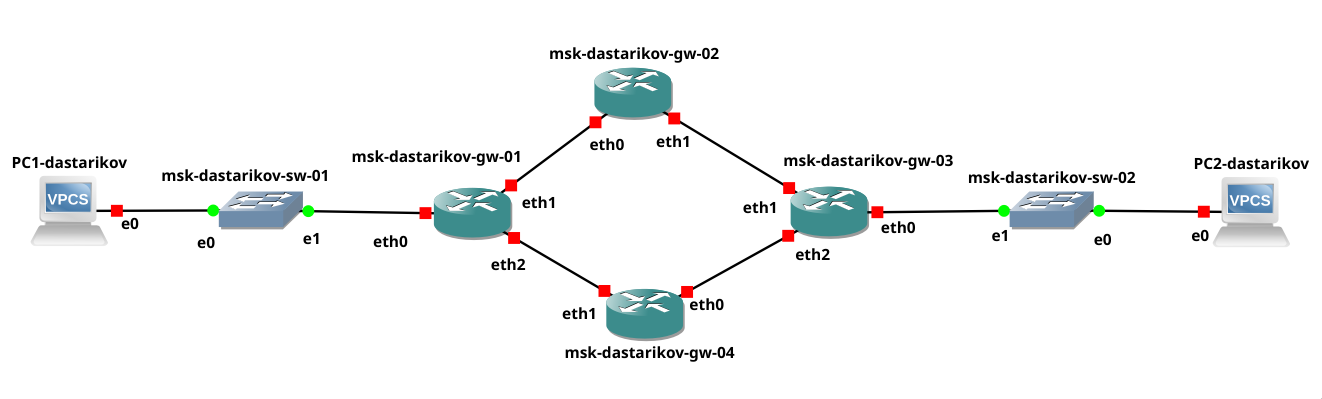
\includegraphics[width=0.8\textwidth]{../images/image00.png}
    \captionof{figure}{Топология сети.}
    \label{00}
  \end{center}

\textbf{Топология моделируемой сети.}
\begin{enumerate}
\item Запустили GNS3 VM и GNS3. Создали новый проект.
\item В рабочем пространстве разместили и соединили устройства в соответствии с топологией, приведённой на рис. \ref{00}. Использовали маршрутизаторы FRR.
\item Изменили отображаемые названия устройств. Коммутаторам присвоили названия по принципу \texttt{msk-dastarikov-sw-0x}, маршрутизаторам — по принципу \texttt{msk-dastarikov-gw-0x}, VPCS — по принципу \texttt{PCx-dastarikov}, где вместо x — порядковый номер устройства.
\item Включили захват трафика на соединении между коммутатором \texttt{sw-01} и маршрутизатором \texttt{gw-01}, а также между коммутатором \texttt{sw-02} и маршрутизатором \texttt{gw-03}.

\item Присвоили IPv4-адреса оконечным устройствам PC1 и PC2 в соответствии с данными в табл. \ref{tab2} (рис. \ref{01} и \ref{02}):
  PC1:
\begin{minted}{bash}
  ip 10.0.10.10/24 10.0.10.1
  save
  show ip
\end{minted}
  PC2:
\begin{minted}{bash}
  ip 10.0.11.10/24 10.0.11.1
  save
  show ip
\end{minted}

  \begin{center}
    \centering
    
\includegraphics[width=0.8\textwidth]{../images/image01.png}
    \captionof{figure}{Настройка IP-адреса PC1.}
    \label{01}
  \end{center}

  \begin{center}
    \centering
    
\includegraphics[width=0.8\textwidth]{../images/image02.png}
    \captionof{figure}{Настройка IP-адреса PC2.}
    \label{02}
  \end{center}

\item Настройте IPv4-адреса на интерфейсах маршрутизаторов (рис. \ref{03}-\ref{10}):
  msk-dastarikov-gw-01:
\begin{minted}{bash}
    frr# configure terminal
    frr(config)# hostname msk-dastarikov-gw-01
    msk-dastarikov-gw-01(config)# interface eth0
    msk-dastarikov-gw-01(config-if)# ip address 10.0.10.1/24
    msk-dastarikov-gw-01(config-if)# no shutdown
    msk-dastarikov-gw-01(config-if)# exit
    msk-dastarikov-gw-01(config)# interface eth1
    msk-dastarikov-gw-01(config-if)# ip address 10.0.1.1/24
    msk-dastarikov-gw-01(config-if)# no shutdown
    msk-dastarikov-gw-01(config-if)# exit
    msk-dastarikov-gw-01(config)# interface eth2
    msk-dastarikov-gw-01(config-if)# ip address 10.0.4.2/24
    msk-dastarikov-gw-01(config-if)# no shutdown
    msk-dastarikov-gw-01(config-if)# exit
    msk-dastarikov-gw-01(config)# exit
    msk-dastarikov-gw-01# write memory
    msk-dastarikov-gw-01# show running-config
\end{minted}
  msk-dastarikov-gw-02:
\begin{minted}{bash}
    frr# configure terminal
    frr(config)# hostname msk-dastarikov-gw-02
    msk-dastarikov-gw-02(config)# interface eth0
    msk-dastarikov-gw-02(config-if)# ip address 10.0.1.2/24
    msk-dastarikov-gw-02(config-if)# no shutdown
    msk-dastarikov-gw-02(config-if)# exit
    msk-dastarikov-gw-02(config)# interface eth1
    msk-dastarikov-gw-02(config-if)# ip address 10.0.2.1/24
    msk-dastarikov-gw-02(config-if)# no shutdown
    msk-dastarikov-gw-02(config-if)# exit
    msk-dastarikov-gw-02(config)# exit
    msk-dastarikov-gw-02# write memory
    msk-dastarikov-gw-02# show running-config
\end{minted}
  msk-dastarikov-gw-03:
\begin{minted}{bash}
    frr# configure terminal
    frr(config)# hostname msk-dastarikov-gw-03
    msk-dastarikov-gw-03(config)# interface eth0
    msk-dastarikov-gw-03(config-if)# ip address 10.0.11.1/24
    msk-dastarikov-gw-03(config-if)# no shutdown
    msk-dastarikov-gw-03(config-if)# exit
    msk-dastarikov-gw-03(config)# interface eth1
    msk-dastarikov-gw-03(config-if)# ip address 10.0.2.2/24
    msk-dastarikov-gw-03(config-if)# no shutdown
    msk-dastarikov-gw-03(config-if)# exit
    msk-dastarikov-gw-03(config)# interface eth2
    msk-dastarikov-gw-03(config-if)# ip address 10.0.3.1/24
    msk-dastarikov-gw-03(config-if)# no shutdown
    msk-dastarikov-gw-03(config-if)# exit
    msk-dastarikov-gw-03(config)# exit
    msk-dastarikov-gw-03# write memory
    msk-dastarikov-gw-03# show running-config
\end{minted}
  msk-dastarikov-gw-04:
\begin{minted}{bash}
    frr# configure terminal
    frr(config)# hostname msk-dastarikov-gw-04
    msk-dastarikov-gw-04(config)# interface eth0
    msk-dastarikov-gw-04(config-if)# ip address 10.0.3.2/24
    msk-dastarikov-gw-04(config-if)# no shutdown
    msk-dastarikov-gw-04(config-if)# exit
    msk-dastarikov-gw-04(config)# interface eth1
    msk-dastarikov-gw-04(config-if)# ip address 10.0.4.1/24
    msk-dastarikov-gw-04(config-if)# no shutdown
    msk-dastarikov-gw-04(config-if)# exit
    msk-dastarikov-gw-04(config)# exit
    msk-dastarikov-gw-04# write memory
    msk-dastarikov-gw-04# show running-config
\end{minted}

  \begin{center}
    \centering
    
\includegraphics[width=0.8\textwidth]{../images/image03.png}
    \captionof{figure}{Настройка адресации на маршрутизаторе \texttt{gw-01}.}
    \label{03}
  \end{center}

  \begin{center}
    \centering
    
\includegraphics[width=0.6\textwidth]{../images/image04.png}
    \captionof{figure}{Просмотр конфига маршрутизатора \texttt{gw-01}.}
    \label{04}
  \end{center}


  \begin{center}
    \centering
    
\includegraphics[width=0.8\textwidth]{../images/image05.png}
    \captionof{figure}{Настройка адресации на маршрутизаторе \texttt{gw-02}.}
    \label{05}
  \end{center}

  \begin{center}
    \centering
    
\includegraphics[width=0.8\textwidth]{../images/image06.png}
    \captionof{figure}{Просмотр конфига маршрутизатора \texttt{gw-02}.}
    \label{06}
  \end{center}

  \begin{center}
    \centering
    
\includegraphics[width=0.6\textwidth]{../images/image07.png}
    \captionof{figure}{Настройка адресации на маршрутизаторе \texttt{gw-03}.}
    \label{07}
  \end{center}

  \begin{center}
    \centering
    
\includegraphics[width=0.8\textwidth]{../images/image08.png}
    \captionof{figure}{Просмотр конфига маршрутизатора \texttt{gw-03}.}
    \label{08}
  \end{center}

  \begin{center}
    \centering
    
\includegraphics[width=0.8\textwidth]{../images/image09.png}
    \captionof{figure}{Настройка адресации на маршрутизаторе \texttt{gw-04}.}
    \label{09}
  \end{center}

  \begin{center}
    \centering
    
\includegraphics[width=0.8\textwidth]{../images/image10.png}
    \captionof{figure}{Просмотр конфига маршрутизатора \texttt{gw-04}.}
    \label{10}
  \end{center}

\item Присвоили IPv6-адреса оконечным устройствам PC1 и PC2 в соответствии с данными в табл. \ref{tab2}(рис. \ref{11} и \ref{12}):
  PC1:
\begin{minted}{bash}
  ip 2001:10::a/64
  save
  show ipv6
\end{minted}
  PC2:
\begin{minted}{bash}
  ip 2001:11::a/64
  save
  show ipv6
\end{minted}

  \begin{center}
    \centering
    
\includegraphics[width=0.8\textwidth]{../images/image11.png}
    \captionof{figure}{Настройка IPv6-адреса PC1.}
    \label{11}
  \end{center}

  \begin{center}
    \centering
    
\includegraphics[width=0.8\textwidth]{../images/image12.png}
    \captionof{figure}{Настройка IPv6-адреса PC2.}
    \label{12}
  \end{center}

\item Настроили IPv6-адреса на интерфейсах маршрутизаторов (рис. \ref{13}-\ref{20}):
\begin{minted}{bash}
    msk-dastarikov-gw-01:
    msk-dastarikov-gw-01# configure terminal
    msk-dastarikov-gw-01(config)# ipv6 forwarding
    msk-dastarikov-gw-01(config)# interface eth0
    msk-dastarikov-gw-01(config-if)# ipv6 address 2001:10::1/64
    msk-dastarikov-gw-01(config-if)# no ipv6 nd suppress-ra
    msk-dastarikov-gw-01(config-if)# ipv6 nd prefix 2001:10::/64
    msk-dastarikov-gw-01(config-if)# no shutdown
    msk-dastarikov-gw-01(config-if)# exit
    msk-dastarikov-gw-01(config)# interface eth1
    msk-dastarikov-gw-01(config-if)# ipv6 address 2001:1::1/64
    msk-dastarikov-gw-01(config-if)# no shutdown
    msk-dastarikov-gw-01(config-if)# exit
    msk-dastarikov-gw-01(config)# interface eth2
    msk-dastarikov-gw-01(config-if)# ipv6 address 2001:4::2/64
    msk-dastarikov-gw-01(config-if)# no shutdown
    msk-dastarikov-gw-01(config-if)# exit
    msk-dastarikov-gw-01(config)# exit
    msk-dastarikov-gw-01# write memory
    msk-dastarikov-gw-01# show running-config
\end{minted}
  msk-dastarikov-gw-02:
\begin{minted}{bash}
    msk-dastarikov-gw-02# configure terminal
    msk-dastarikov-gw-02(config)# ipv6 forwarding
    msk-dastarikov-gw-02(config)# interface eth0
    msk-dastarikov-gw-02(config-if)# ipv6 address 2001:1::2/64
    msk-dastarikov-gw-02(config-if)# no shutdown
    msk-dastarikov-gw-02(config-if)# exit
    msk-dastarikov-gw-02(config)# interface eth1
    msk-dastarikov-gw-02(config-if)# ipv6 address 2001:2::1/64
    msk-dastarikov-gw-02(config-if)# no shutdown
    msk-dastarikov-gw-02(config-if)# exit
    msk-dastarikov-gw-02(config)# exit
    msk-dastarikov-gw-02# write memory
    msk-dastarikov-gw-02# show running-config
\end{minted}
  msk-dastarikov-gw-03:
\begin{minted}{bash}
    msk-dastarikov-gw-03# configure terminal
    msk-dastarikov-gw-03(config)# ipv6 forwarding
    msk-dastarikov-gw-03(config)# interface eth0
    msk-dastarikov-gw-03(config-if)# ipv6 address 2001:11::1/64
    msk-dastarikov-gw-03(config-if)# no ipv6 nd suppress-ra
    msk-dastarikov-gw-03(config-if)# ipv6 nd prefix 2001:11::/64
    msk-dastarikov-gw-03(config-if)# no shutdown
    msk-dastarikov-gw-03(config-if)# exit
    msk-dastarikov-gw-03(config)# interface eth1
    msk-dastarikov-gw-03(config-if)# ipv6 address 2001:2::2/64
    msk-dastarikov-gw-03(config-if)# no shutdown
    msk-dastarikov-gw-03(config-if)# exit
    msk-dastarikov-gw-03(config)# interface eth2
    msk-dastarikov-gw-03(config-if)# ipv6 address 2001:3::1/64
    msk-dastarikov-gw-03(config-if)# no shutdown
    msk-dastarikov-gw-03(config-if)# exit
    msk-dastarikov-gw-03(config)# exit
    msk-dastarikov-gw-03# write memory
    msk-dastarikov-gw-03# show running-confi
\end{minted}
  msk-dastarikov-gw-04:
\begin{minted}{bash}
    msk-dastarikov-gw-04# configure terminal
    msk-dastarikov-gw-04(config)# ipv6 forwarding
    msk-dastarikov-gw-04(config)# interface eth0
    msk-dastarikov-gw-04(config-if)# ipv6 address 2001:3::2/64
    msk-dastarikov-gw-04(config-if)# no shutdown
    msk-dastarikov-gw-04(config-if)# exit
    msk-dastarikov-gw-04(config)# interface eth1
    msk-dastarikov-gw-04(config-if)# ipv6 address 2001:4::1/64
    msk-dastarikov-gw-04(config-if)# no shutdown
    msk-dastarikov-gw-04(config-if)# exit
    msk-dastarikov-gw-04(config)# exit
    msk-dastarikov-gw-04# write memory
    msk-dastarikov-gw-04# show running-config
\end{minted}

  \begin{center}
    \centering
    
\includegraphics[width=0.8\textwidth]{../images/image13.png}
    \captionof{figure}{Настройка IPv6-адресации на маршрутизаторе \texttt{gw-01}.}
    \label{13}
  \end{center}

  \begin{center}
    \centering
    
\includegraphics[width=0.8\textwidth]{../images/image14.png}
    \captionof{figure}{Просмотр конфига маршрутизатора \texttt{gw-01}.}
    \label{14}
  \end{center}


  \begin{center}
    \centering
    
\includegraphics[width=0.8\textwidth]{../images/image15.png}
    \captionof{figure}{Настройка IPv6-адресации на маршрутизаторе \texttt{gw-02}.}
    \label{15}
  \end{center}

  \begin{center}
    \centering
    
\includegraphics[width=0.8\textwidth]{../images/image16.png}
    \captionof{figure}{Просмотр конфига маршрутизатора \texttt{gw-02}.}
    \label{16}
  \end{center}

  \begin{center}
    \centering
    
\includegraphics[width=0.8\textwidth]{../images/image17.png}
    \captionof{figure}{Настройка IPv6-адресации на маршрутизаторе \texttt{gw-03}.}
    \label{17}
  \end{center}

  \begin{center}
    \centering
    
\includegraphics[width=0.8\textwidth]{../images/image18.png}
    \captionof{figure}{Просмотр конфига маршрутизатора \texttt{gw-03}.}
    \label{18}
  \end{center}

  \begin{center}
    \centering
    
\includegraphics[width=0.8\textwidth]{../images/image19.png}
    \captionof{figure}{Настройка IPv6-адресации на маршрутизаторе \texttt{gw-04}.}
    \label{19}
  \end{center}

  \begin{center}
    \centering
    
\includegraphics[width=0.8\textwidth]{../images/image20.png}
    \captionof{figure}{Просмотр конфига маршрутизатора \texttt{gw-04}.}
    \label{20}
  \end{center}
\end{enumerate}

\textbf{Настройка динамической маршрутизации по протоколу RIP.}
\begin{enumerate}
\item На маршрутизаторах настроили RIP в качестве протокола динамической маршрутизации (рис. \ref{21}-\ref{24}):
\begin{minted}{bash}
    msk-dastarikov-gw-01:
    msk-dastarikov-gw-01# configure terminal
    msk-dastarikov-gw-01(config)# router rip
    msk-dastarikov-gw-01(config-router)# version 2
    msk-dastarikov-gw-01(config-router)# network eth0
    msk-dastarikov-gw-01(config-router)# network eth1
    msk-dastarikov-gw-01(config-router)# network eth2
    msk-dastarikov-gw-01(config-router)# exit
    msk-dastarikov-gw-01(config)# exit
    msk-dastarikov-gw-01# write memory
\end{minted}
    msk-dastarikov-gw-02:
\begin{minted}{bash}
    msk-dastarikov-gw-02# configure terminal
    msk-dastarikov-gw-02(config)# router rip
    msk-dastarikov-gw-02(config-router)# version 2
    msk-dastarikov-gw-02(config-router)# network eth0
    msk-dastarikov-gw-02(config-router)# network eth1
    msk-dastarikov-gw-02(config-router)# exit
    msk-dastarikov-gw-02(config)# exit
    msk-dastarikov-gw-02# write memory
\end{minted}
    msk-dastarikov-gw-03:
\begin{minted}{bash}
    msk-dastarikov-gw-03# configure terminal
    msk-dastarikov-gw-03(config)# router rip
    msk-dastarikov-gw-03(config-router)# version 2
    msk-dastarikov-gw-03(config-router)# network eth0
    msk-dastarikov-gw-03(config-router)# network eth1
    msk-dastarikov-gw-03(config-router)# network eth2
    msk-dastarikov-gw-03(config-router)# exit
    msk-dastarikov-gw-03(config)# exit
    msk-dastarikov-gw-03# write memory
\end{minted}
    msk-dastarikov-gw-04:
\begin{minted}{bash}
    msk-dastarikov-gw-04# configure terminal
    msk-dastarikov-gw-04(config)# router rip
    msk-dastarikov-gw-04(config-router)# version 2
    msk-dastarikov-gw-04(config-router)# network eth0
    msk-dastarikov-gw-04(config-router)# network eth1
    msk-dastarikov-gw-04(config-router)# exit
    msk-dastarikov-gw-04(config)# exit
    msk-dastarikov-gw-04# write memory
\end{minted}

    \begin{center}
      \centering
      
\includegraphics[width=0.8\textwidth]{../images/image21.png}
      \captionof{figure}{Настройка протокола RIP на маршрутизатору \texttt{gw-01}.}
      \label{21}
    \end{center}

    \begin{center}
      \centering
      
\includegraphics[width=0.8\textwidth]{../images/image22.png}
      \captionof{figure}{Настройка протокола RIP на маршрутизатору \texttt{gw-02}.}
      \label{22}
    \end{center}

    \begin{center}
      \centering
      
\includegraphics[width=0.8\textwidth]{../images/image23.png}
      \captionof{figure}{Настройка протокола RIP на маршрутизатору \texttt{gw-03}.}
      \label{23}
    \end{center}

    \begin{center}
      \centering
      
\includegraphics[width=0.8\textwidth]{../images/image24.png}
      \captionof{figure}{Настройка протокола RIP на маршрутизатору \texttt{gw-04}.}
      \label{24}
    \end{center}

  \item Убедились, что маршрутизация по RIP настроена (рис. \ref{25}-\ref{27}):
\begin{minted}{bash}
      msk-dastarikov-gw-01# show ip route rip
      msk-dastarikov-gw-01# show ip rip
      msk-dastarikov-gw-01# show ip rip status
\end{minted}

    \begin{center}
      \centering
      
\includegraphics[width=0.8\textwidth]{../images/image25.png}
      \captionof{figure}{Просмотр настроек маршрутизации по RIP.}
      \label{25}
    \end{center}

    \begin{center}
      \centering
      
\includegraphics[width=0.8\textwidth]{../images/image26.png}
      \captionof{figure}{Просмотр настроек маршрутизации по RIP.}
      \label{26}
    \end{center}

    \begin{center}
      \centering
      
\includegraphics[width=0.8\textwidth]{../images/image27.png}
      \captionof{figure}{Просмотр настроек маршрутизации по RIP.}
      \label{27}
    \end{center}

  \item Проверили пути прохождения пакетов:
    \begin{itemize}
    \item С PC1 пропинговали PC2 и определили путь следования пакетов (рис. \ref{28}):
\begin{minted}{bash}
        PC1> ping 10.0.11.10
        PC1> trace 10.0.11.10 -P 6
\end{minted}

      \begin{center}
        \centering
        
\includegraphics[width=0.8\textwidth]{../images/image28.png}
        \captionof{figure}{Отправка эхо-запроса с PC1 к PC2.}
        \label{28}
      \end{center}

    \item Проверили метрики протокола RIP (рис. \ref{29}):
\begin{minted}{bash}
          msk-dastarikov-gw-01# show ip rip
\end{minted}

      \begin{center}
        \centering
        
\includegraphics[width=0.8\textwidth]{../images/image29.png}
        \captionof{figure}{Просмотр метрик протокола RIP.}
        \label{29}
      \end{center}

    \item Отключили на маршрутизаторе \texttt{msk-dastarikov-gw-02} интерфейс (рис. \ref{30}):
\begin{minted}{bash}
          msk-dastarikov-gw-02# configure terminal
          msk-dastarikov-gw-02(config)# interface eth0
          msk-dastarikov-gw-02(config-if)# shutdown
\end{minted}

      \begin{center}
        \centering
        
\includegraphics[width=0.8\textwidth]{../images/image30.png}
        \captionof{figure}{Отключение на маршрутизаторе \texttt{msk-dastarikov-gw-02} интерфейса \texttt{eth0}.}
        \label{30}
      \end{center}

    \item Проверили метрики протокола RIP (рис. \ref{31}):
\begin{minted}{bash}
          msk-dastarikov-gw-01# show ip rip
\end{minted}

      \begin{center}
        \centering
        
\includegraphics[width=0.8\textwidth]{../images/image31.png}
        \captionof{figure}{Просмотр метрики RIP после сразу отключения маршрутизатора.}
        \label{31}
      \end{center}

    \item С PC1 пропинговали PC2 и определили путь следования пакетов (рис. \ref{32} и \ref{33}). Маршрут восстановился примерно в течение 3х минут.
      
      \begin{center}
        \centering
        
\includegraphics[width=0.8\textwidth]{../images/image32.png}
        \captionof{figure}{Отправка эхо-запроса с PC1 к PC2 по новому маршруту.}
        \label{32}
      \end{center}

      \begin{center}
        \centering
        
\includegraphics[width=0.8\textwidth]{../images/image33.png}
        \captionof{figure}{Просмотр метрики RIP после восстановления маршрута сразу отключения.}
        \label{33}
      \end{center}

    \item Включили на маршрутизаторе \texttt{msk-dastarikov-gw-02} интерфейс:
\begin{minted}{bash}
          msk-dastarikov-gw-02# configure terminal
          msk-dastarikov-gw-02(config)# interface eth0
          msk-dastarikov-gw-02(config-if)# no shutdown
\end{minted}
      
    \item С PC1 пропинговали PC2 и определили путь следования пакетов.
    \end{itemize}

  \item На маршрутизаторах настроили RIPng для сетей IPv6 (рис. \ref{34}-\ref{37}):
\begin{minted}{bash}
      msk-dastarikov-gw-01:
      msk-dastarikov-gw-01# configure terminal
      msk-dastarikov-gw-01(config)# router ripng
      msk-dastarikov-gw-01(config-router)# network eth0
      msk-dastarikov-gw-01(config-router)# network eth1
      msk-dastarikov-gw-01(config-router)# network eth2
      msk-dastarikov-gw-01(config-router)# exit
      msk-dastarikov-gw-01(config)# exit
      msk-dastarikov-gw-01# write memory
\end{minted}
    msk-dastarikov-gw-02:
\begin{minted}{bash}
      msk-dastarikov-gw-02# configure terminal
      msk-dastarikov-gw-02(config)# router ripng
      msk-dastarikov-gw-02(config-router)# network eth0
      msk-dastarikov-gw-02(config-router)# network eth1
      msk-dastarikov-gw-02(config-router)# exit
      msk-dastarikov-gw-02(config)# exit
      msk-dastarikov-gw-02# write memory
\end{minted}
    msk-dastarikov-gw-03:
\begin{minted}{bash}
      msk-dastarikov-gw-03# configure terminal
      msk-dastarikov-gw-03(config)# router ripng
      msk-dastarikov-gw-03(config-router)# network eth0
      msk-dastarikov-gw-03(config-router)# network eth1
      msk-dastarikov-gw-03(config-router)# network eth2
      msk-dastarikov-gw-03(config-router)# exit
      msk-dastarikov-gw-03(config)# exit
      msk-dastarikov-gw-03# write memory
\end{minted}
    msk-dastarikov-gw-04:
\begin{minted}{bash}
      msk-dastarikov-gw-04# configure terminal
      msk-dastarikov-gw-04(config)# router ripng
      msk-dastarikov-gw-04(config-router)# network eth0
      msk-dastarikov-gw-04(config-router)# network eth1
      msk-dastarikov-gw-04(config-router)# exit
      msk-dastarikov-gw-04(config)# exit
      msk-dastarikov-gw-04# write memory
\end{minted}

    \begin{center}
      \centering
      
\includegraphics[width=0.8\textwidth]{../images/image34.png}
      \captionof{figure}{Настройка протокола RIPng на маршрутизатору \texttt{gw-01}.}
      \label{34}
    \end{center}

    \begin{center}
      \centering
      
\includegraphics[width=0.8\textwidth]{../images/image35.png}
      \captionof{figure}{Настройка протокола RIPng на маршрутизатору \texttt{gw-02}.}
      \label{35}
    \end{center}

    \begin{center}
      \centering
      
\includegraphics[width=0.8\textwidth]{../images/image36.png}
      \captionof{figure}{Настройка протокола RIPng на маршрутизатору \texttt{gw-03}.}
      \label{36}
    \end{center}

    \begin{center}
      \centering
      
\includegraphics[width=0.8\textwidth]{../images/image37.png}
      \captionof{figure}{Настройка протокола RIPng на маршрутизатору \texttt{gw-04}.}
      \label{37}
    \end{center}

  \item Проверили пути прохождения пакетов:
    \begin{itemize}
    \item С PC1 пропинговали PC2 и определили путь следования пакетов (рис. \ref{38}):
\begin{minted}{bash}
    PC1> ping 2001:11::a
    PC1> trace 2001:11::a
\end{minted}
      
      \begin{center}
        \centering
        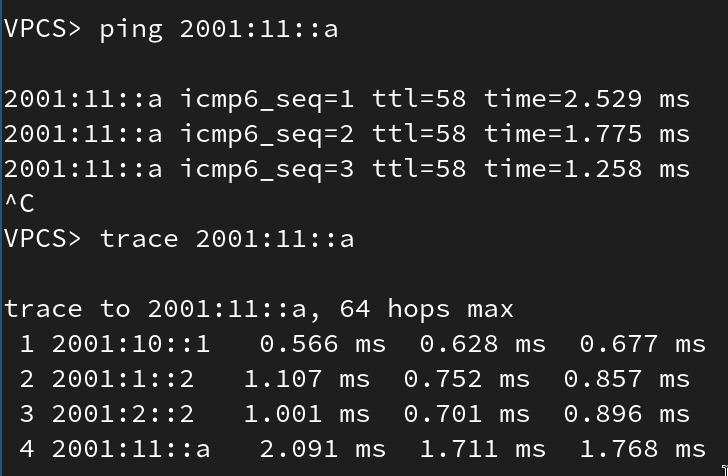
\includegraphics[width=0.8\textwidth]{../images/image38.png}
        \captionof{figure}{Отправка эхо-запроса с PC1 к PC2.}
        \label{38}
      \end{center}

    \item Проверили метрики протокола RIPng (рис. \ref{39}):
\begin{minted}{bash}
        msk-dastarikov-gw-01# show ipv6 ripng
\end{minted}
      
      \begin{center}
        \centering
        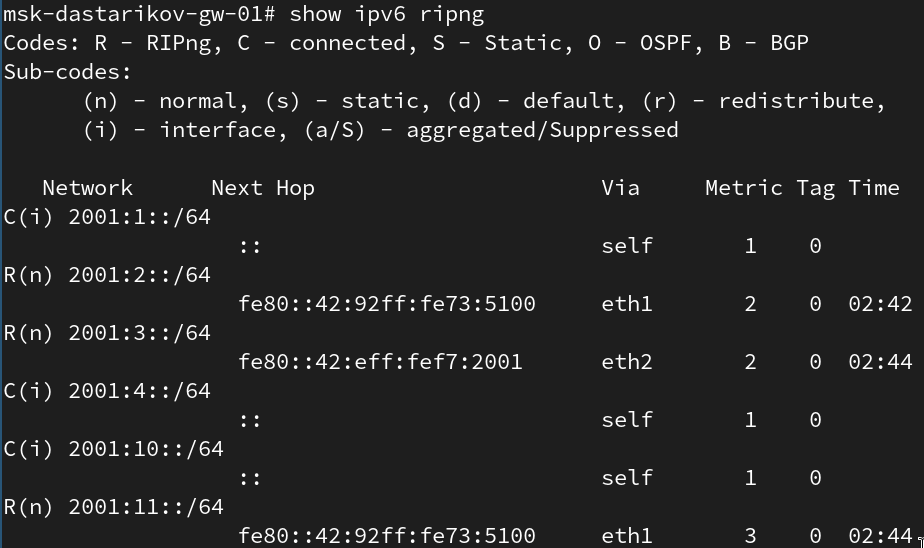
\includegraphics[width=0.8\textwidth]{../images/image39.png}
        \captionof{figure}{Проверка метрики протокола RIPng.}
        \label{39}
      \end{center}


    \item Отключили на маршрутизаторе \texttt{msk-dastarikov-gw-02} интерфейс (рис. \ref{40}):
\begin{minted}{bash}
        msk-dastarikov-gw-02# configure terminal
        msk-dastarikov-gw-02(config)# interface eth0
        msk-dastarikov-gw-02(config-if)# shutdown
\end{minted}

      \begin{center}
        \centering
        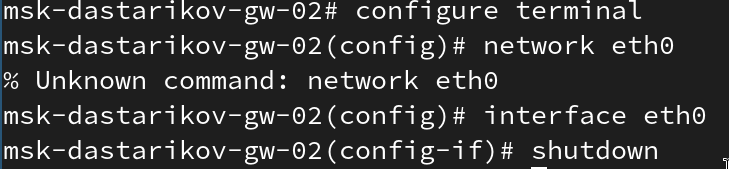
\includegraphics[width=0.8\textwidth]{../images/image40.png}
        \captionof{figure}{Отключение на маршрутизаторе \texttt{msk-dastarikov-gw-02} интерфейса \texttt{eth0}.}
        \label{40}
      \end{center}

    \item Проверили метрики протокола RIPng (рис. \ref{39}):
\begin{minted}{bash}
        msk-dastarikov-gw-01# show ipv6 ripng
\end{minted}

      \begin{center}
        \centering
        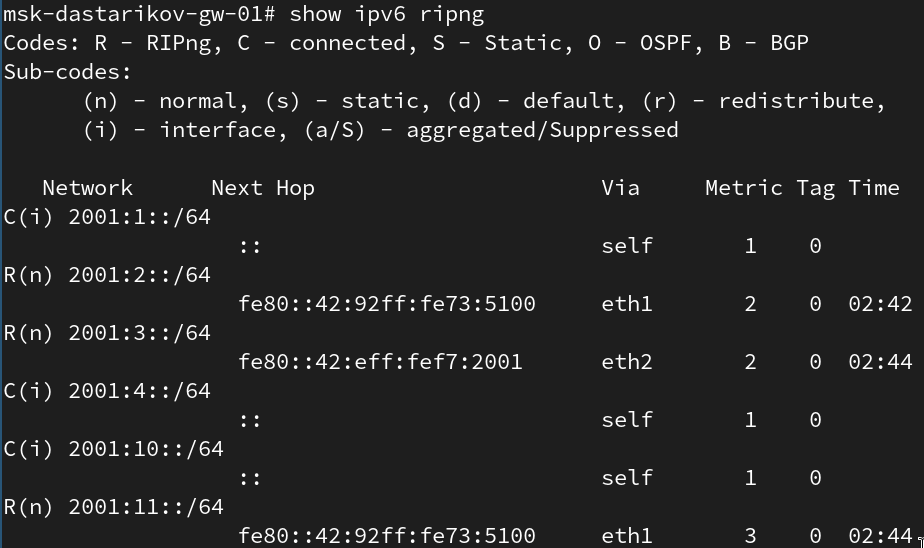
\includegraphics[width=0.8\textwidth]{../images/image39.png}
        \captionof{figure}{Проверка метрики протокола RIPng.}
        \label{39}
      \end{center}

    \item После отключения маршрут между PC1 и PC2 не восстановился, причину найти не удалось.
      
    \item Включили на маршрутизаторе \texttt{msk-dastarikov-gw-02} интерфейс:
\begin{minted}{bash}
        msk-dastarikov-gw-02# configure terminal
        msk-dastarikov-gw-02(config)# interface eth0
        msk-dastarikov-gw-02(config-if)# no shutdown
\end{minted}
    \end{itemize}
  \end{enumerate}

  \textbf{Настройка динамической маршрутизации по протоколу OSPF.}

  \begin{enumerate}
  \item На маршрутизаторах настроили OSPFv2 для сетей IPv4 (рис. \ref{41}-\ref{44}):
\begin{minted}{bash}
    msk-dastarikov-gw-01:
    msk-dastarikov-gw-01# configure terminal
    msk-dastarikov-gw-01(config)# router ospf
    msk-dastarikov-gw-01(config-router)# network 10.0.10.0/24 area 0.0.0.0
    msk-dastarikov-gw-01(config-router)# network 10.0.1.0/24 area  0.0.0.0
    msk-dastarikov-gw-01(config-router)# network 10.0.4.0/24 area 0.0.0.0
    msk-dastarikov-gw-01(config-router)# exit
    msk-dastarikov-gw-01(config)# exit
    msk-dastarikov-gw-01# write memory
\end{minted}
    msk-dastarikov-gw-02:
\begin{minted}{bash}
    msk-dastarikov-gw-02# configure terminal
    msk-dastarikov-gw-02(config)# router ospf
    msk-dastarikov-gw-02(config-router)# network 10.0.1.0/24 area 0.0.0.0
    msk-dastarikov-gw-02(config-router)# network 10.0.2.0/24 area 0.0.0.0
    msk-dastarikov-gw-02(config-router)# exit
    msk-dastarikov-gw-02(config)# exit
    msk-dastarikov-gw-02# write memory
\end{minted}
    msk-dastarikov-gw-03:
\begin{minted}{bash}
    msk-dastarikov-gw-03# configure terminal
    msk-dastarikov-gw-03(config)# router ospf
    msk-dastarikov-gw-03(config-router)# network 10.0.11.0/24 area 0.0.0.0
    msk-dastarikov-gw-03(config-router)# network 10.0.2.0/24 area 0.0.0.0
    msk-dastarikov-gw-03(config-router)# network 10.0.3.0/24 area 0.0.0.0
    msk-dastarikov-gw-03(config-router)# exit
    msk-dastarikov-gw-03(config)# exit
    msk-dastarikov-gw-03# write memory
\end{minted}
    msk-dastarikov-gw-04:
\begin{minted}{bash}
    msk-dastarikov-gw-04# configure terminal
    msk-dastarikov-gw-04(config)# router ospf
    msk-dastarikov-gw-04(config-router)# network 10.0.3.0/24 area 0.0.0.0
    msk-dastarikov-gw-04(config-router)# network 10.0.4.0/24 area 0.0.0.0
    msk-dastarikov-gw-04(config-router)# exit
    msk-dastarikov-gw-04(config)# exit
    msk-dastarikov-gw-04# write memory
\end{minted}

    \begin{center}
      \centering
      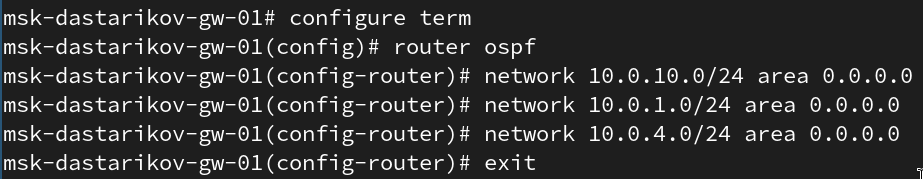
\includegraphics[width=0.8\textwidth]{../images/image41.png}
      \captionof{figure}{Настройка протокола OSPF на маршрутизатору \texttt{gw-01}.}
      \label{41}
    \end{center}

    \begin{center}
      \centering
      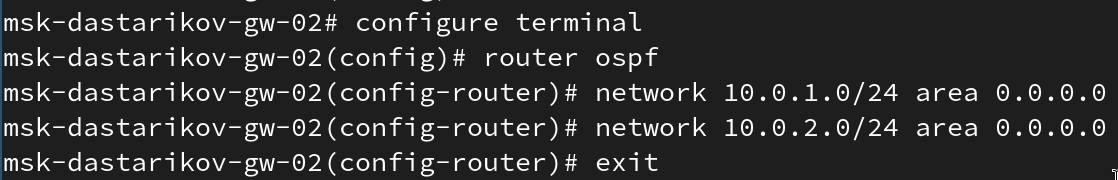
\includegraphics[width=0.8\textwidth]{../images/image42.png}
      \captionof{figure}{Настройка протокола OSPF на маршрутизатору \texttt{gw-02}.}
      \label{42}
    \end{center}

    \begin{center}
      \centering
      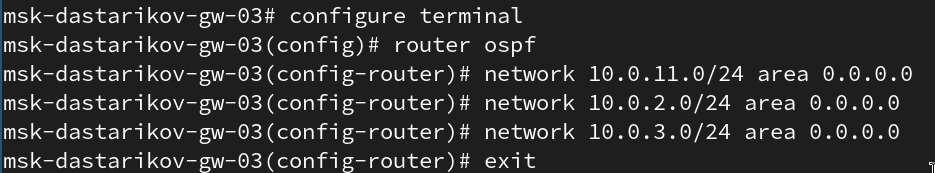
\includegraphics[width=0.8\textwidth]{../images/image43.png}
      \captionof{figure}{Настройка протокола OSPF на маршрутизатору \texttt{gw-03}.}
      \label{43}
    \end{center}

    \begin{center}
      \centering
      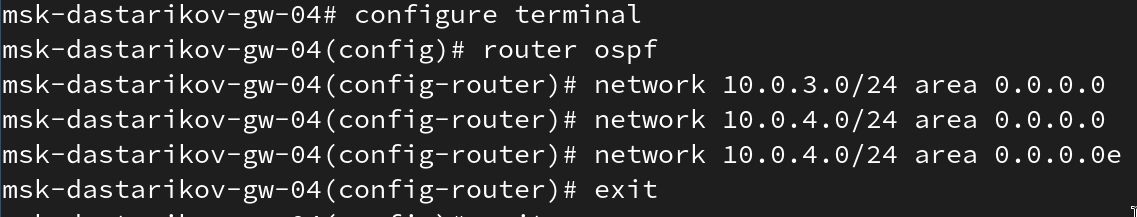
\includegraphics[width=0.8\textwidth]{../images/image44.png}
      \captionof{figure}{Настройка протокола OSPF на маршрутизатору \texttt{gw-04}.}
      \label{44}
    \end{center}


  \item С PC1 пропингуйте PC2 и определите путь следования пакетов (рис. \ref{28}):
\begin{minted}{bash}
    PC1> ping 10.0.11.10
    PC1> trace 10.0.11.10 -P 6
\end{minted}

    \begin{center}
      \centering
      
\includegraphics[width=0.8\textwidth]{../images/image28.png}
      \captionof{figure}{Отправка эхо-запроса с PC1 к PC2.}
      \label{28}
    \end{center}

  \item Проверьте таблицу маршрутизации протокола OSPFv2 (рис. \ref{46}):
\begin{minted}{bash}
    msk-dastarikov-gw-01# show ip ospf neighbor
    msk-dastarikov-gw-01# show ip ospf route
\end{minted}

    \begin{center}
      \centering
      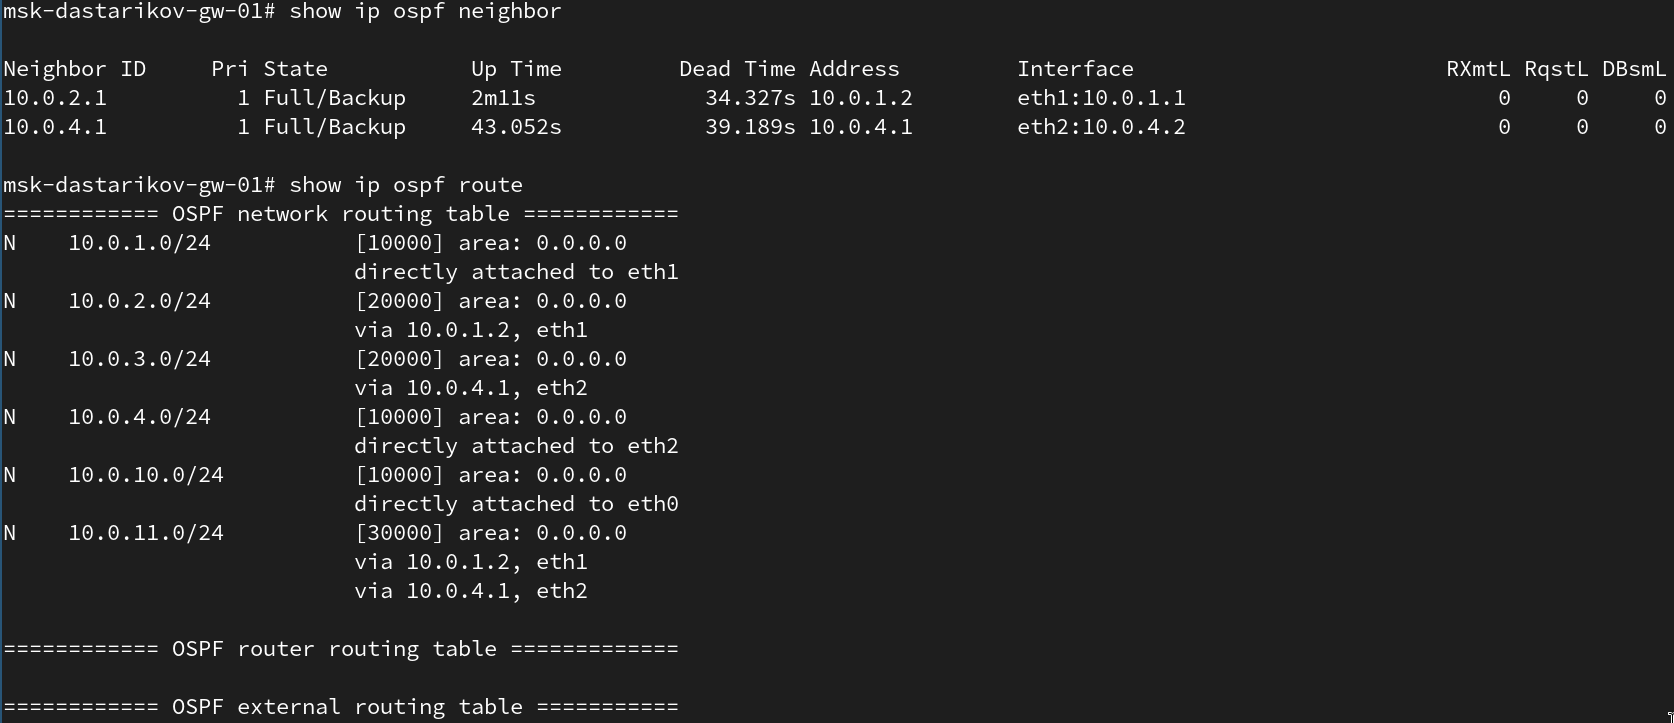
\includegraphics[width=0.8\textwidth]{../images/image46.png}
      \captionof{figure}{Просмотр таблицы маршрутизации протокола OSPFv2.}
      \label{46}
    \end{center}

  \item Отключили на маршрутизаторе \texttt{msk-dastarikov-gw-02} интерфейс (рис. \ref{47}):
\begin{minted}{bash}
    msk-dastarikov-gw-02# configure terminal
    msk-dastarikov-gw-02(config)# interface eth0
    msk-dastarikov-gw-02(config-if)# shutdown
\end{minted}

    \begin{center}
      \centering
      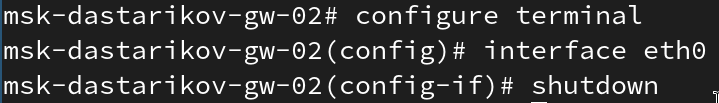
\includegraphics[width=0.8\textwidth]{../images/image47.png}
      \captionof{figure}{Отключение на маршрутизаторе \texttt{msk-dastarikov-gw-02} интерфейса \texttt{eth0}.}
      \label{47}
    \end{center}

  \item Проверили таблицу маршрутизации протокола OSPFv2 (рис. \ref{49}):
\begin{minted}{bash}
    msk-dastarikov-gw-01# show ip ospf neighbor
    msk-dastarikov-gw-01# show ip ospf route
\end{minted}

    \begin{center}
      \centering
      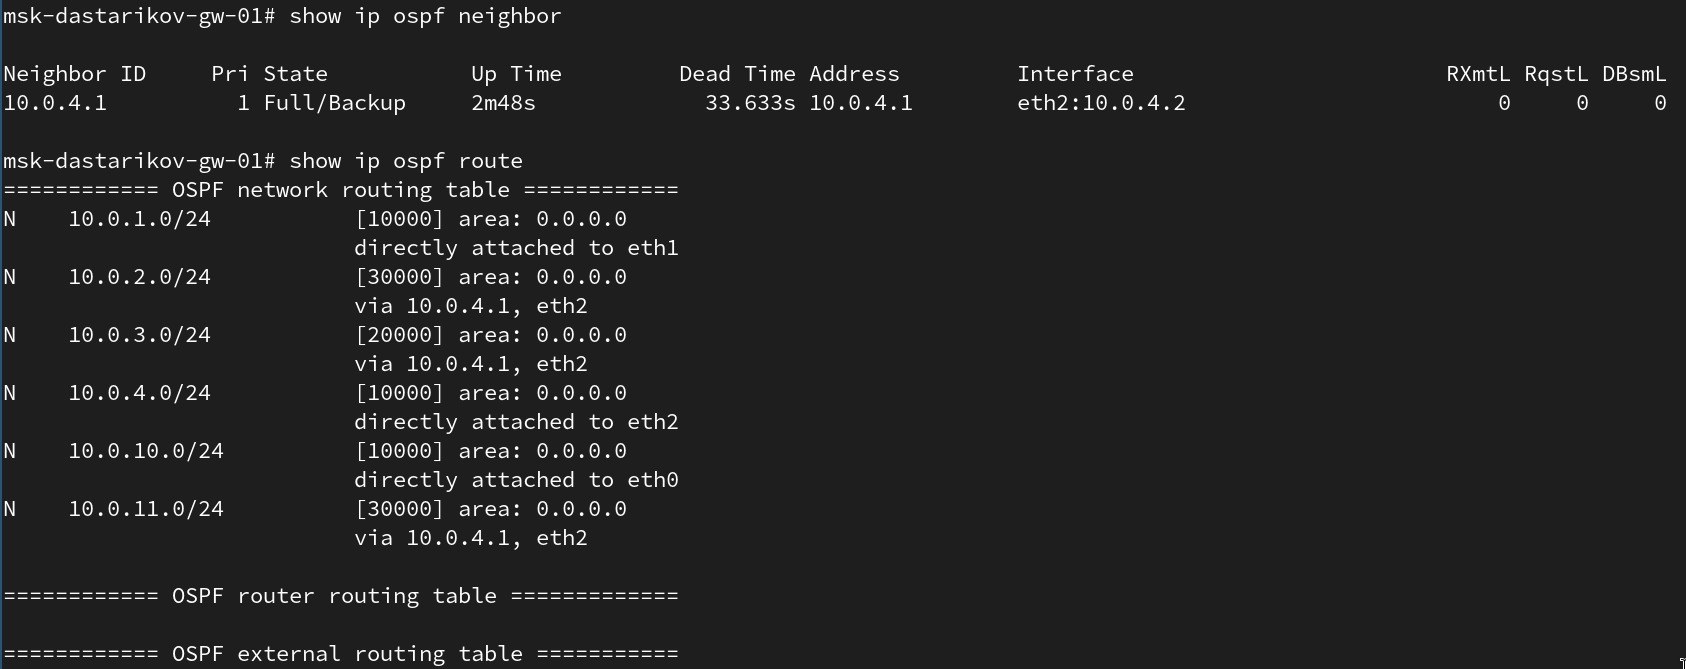
\includegraphics[width=0.8\textwidth]{../images/image49.png}
      \captionof{figure}{Просмотр таблицы маршрутизации протокола OSPFv2 после отключения интерфейса маршрутизатора.}
      \label{49}
    \end{center}

  \item С PC1 пропинговали PC2 и определили путь следования пакетов (рис. \ref{51}). Маршрут восстановился в течение 10 секунд.

    \begin{center}
      \centering
      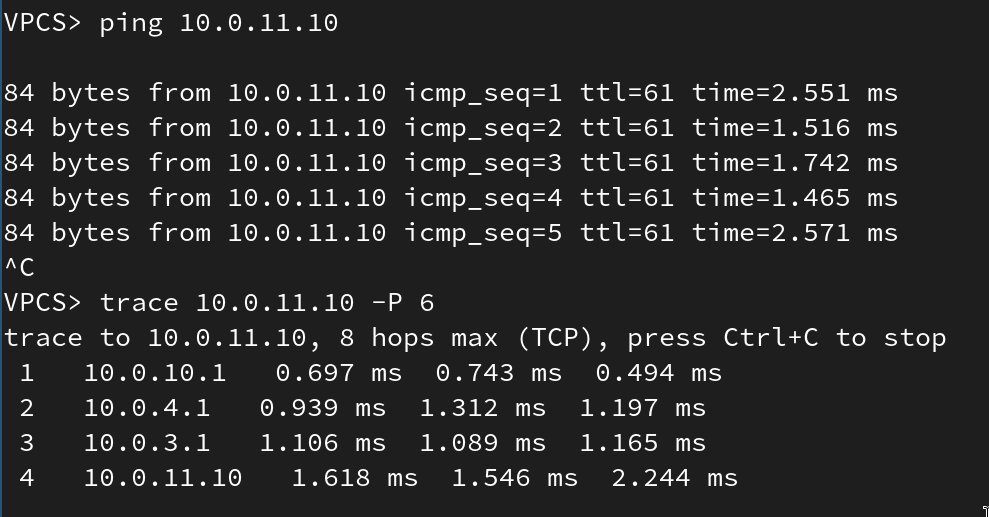
\includegraphics[width=0.8\textwidth]{../images/image51.png}
      \captionof{figure}{Отправка эхо-запроса с PC1 к PC2 после обновления маршрута.}
      \label{51}
    \end{center}

  \item Включили на маршрутизаторе msk-dastarikov-gw-02 интерфейс:
\begin{minted}{bash}
    msk-dastarikov-gw-02# configure terminal
    msk-dastarikov-gw-02(config)# interface eth0
    msk-dastarikov-gw-02(config-if)# no shutdown
\end{minted}

  \item С PC1 пропинговали PC2 и определили путь следования пакетов (рис. \ref{52}).

    \begin{center}
      \centering
      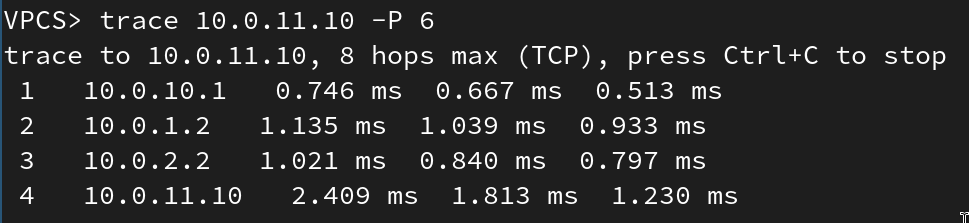
\includegraphics[width=0.8\textwidth]{../images/image52.png}
      \captionof{figure}{Отправка эхо-запроса с PC1 к PC2 после включения обратного интерфейса.}
      \label{52}
    \end{center}

  \item На маршрутизаторах настроили OSPFv3 для сетей IPv6 (рис. \ref{53}-\ref{56}):
\begin{minted}{bash}
    msk-dastarikov-gw-01:
    msk-dastarikov-gw-01# configure terminal
    msk-dastarikov-gw-01(config)# router ospf6
    msk-dastarikov-gw-01(config-rtr)# ospf6 router-id 1.1.1.1
    msk-dastarikov-gw-01(config-rtr)# exit
    msk-dastarikov-gw-01(config)# interface eth0
    msk-dastarikov-gw-01(config-if)# ipv6 ospf6 area 0
    msk-dastarikov-gw-01(config-if)# exit
    msk-dastarikov-gw-01(config)# interface eth1
    msk-dastarikov-gw-01(config-if)# ipv6 ospf6 area 0
    msk-dastarikov-gw-01(config-if)# exit
    msk-dastarikov-gw-01(config)# interface eth2
    msk-dastarikov-gw-01(config-if)# ipv6 ospf6 area 0
    msk-dastarikov-gw-01(config-if)# exit
    msk-dastarikov-gw-01(config)# exit
    msk-dastarikov-gw-01# write memory
\end{minted}
    msk-dastarikov-gw-02:
\begin{minted}{bash}
    msk-dastarikov-gw-02# configure terminal
    msk-dastarikov-gw-02(config)# router ospf6
    msk-dastarikov-gw-02(config-rtr)# ospf6 router-id 2.2.2.2
    msk-dastarikov-gw-02(config-rtr)# exit
    msk-dastarikov-gw-02(config)# interface eth0
    msk-dastarikov-gw-02(config-if)# ipv6 ospf6 area 0
    msk-dastarikov-gw-02(config-if)# exit
    msk-dastarikov-gw-02(config)# interface eth1
    msk-dastarikov-gw-02(config-if)# ipv6 ospf6 area 0
    msk-dastarikov-gw-02(config-if)# exit
    msk-dastarikov-gw-02(config)# exit
    msk-dastarikov-gw-02# write memory
\end{minted}
    msk-dastarikov-gw-03:
\begin{minted}{bash}
    msk-dastarikov-gw-03# configure terminal
    msk-dastarikov-gw-03(config)# router ospf6
    msk-dastarikov-gw-03(config-rtr)# ospf6 router-id 3.3.3.3
    msk-dastarikov-gw-03(config-rtr)# exit
    msk-dastarikov-gw-03(config)# interface eth0
    msk-dastarikov-gw-03(config-if)# ipv6 ospf6 area 0
    msk-dastarikov-gw-03(config-if)# exit
    msk-dastarikov-gw-03(config)# interface eth1
    msk-dastarikov-gw-03(config-if)# ipv6 ospf6 area 0
    msk-dastarikov-gw-03(config-if)# exit
    msk-dastarikov-gw-03(config)# interface eth2
    msk-dastarikov-gw-03(config-if)# ipv6 ospf6 area 0
    msk-dastarikov-gw-03(config-if)# exit
    msk-dastarikov-gw-03(config)# exit
    msk-dastarikov-gw-03# write memory
\end{minted}
    msk-dastarikov-gw-04:
\begin{minted}{bash}
    msk-dastarikov-gw-04# configure terminal
    msk-dastarikov-gw-04(config)# router ospf6
    msk-dastarikov-gw-04(config-rtr)# ospf6 router-id 4.4.4.4
    msk-dastarikov-gw-04(config-rtr)# exit
    msk-dastarikov-gw-04(config)# interface eth0
    msk-dastarikov-gw-04(config-if)# ipv6 ospf6 area 0
    msk-dastarikov-gw-04(config-if)# exit
    msk-dastarikov-gw-04(config)# interface eth1
    msk-dastarikov-gw-04(config-if)# ipv6 ospf6 area 0
    msk-dastarikov-gw-04(config-if)# exit
    msk-dastarikov-gw-04(config)# exit
    msk-dastarikov-gw-04# write memory
\end{minted}

    \begin{center}
      \centering
      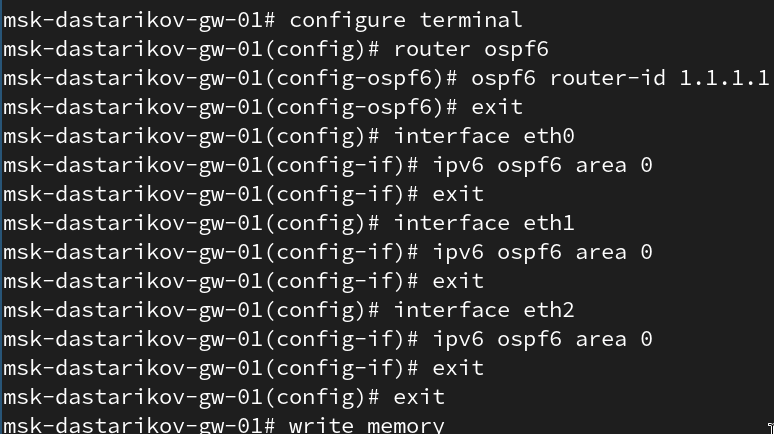
\includegraphics[width=0.8\textwidth]{../images/image53.png}
      \captionof{figure}{Настройка протокола OSPFv3 на маршрутизатору \texttt{gw-01}.}
      \label{53}
    \end{center}

    \begin{center}
      \centering
      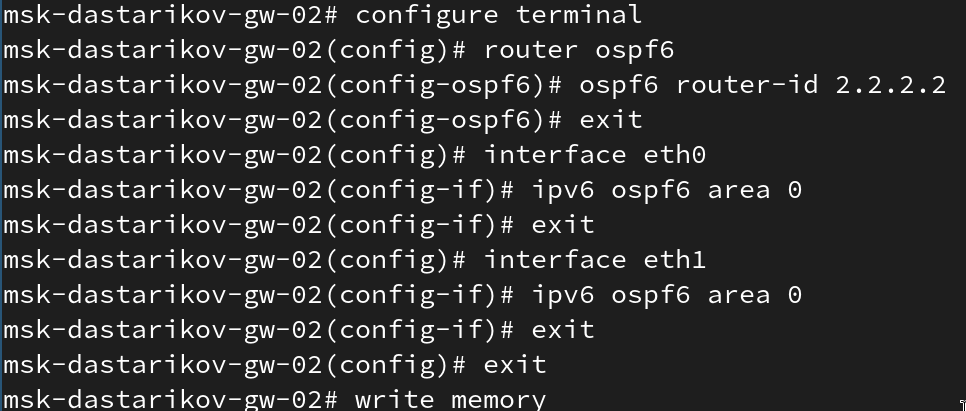
\includegraphics[width=0.8\textwidth]{../images/image54.png}
      \captionof{figure}{Настройка протокола OSPFv3 на маршрутизатору \texttt{gw-02}.}
      \label{54}
    \end{center}

    \begin{center}
      \centering
      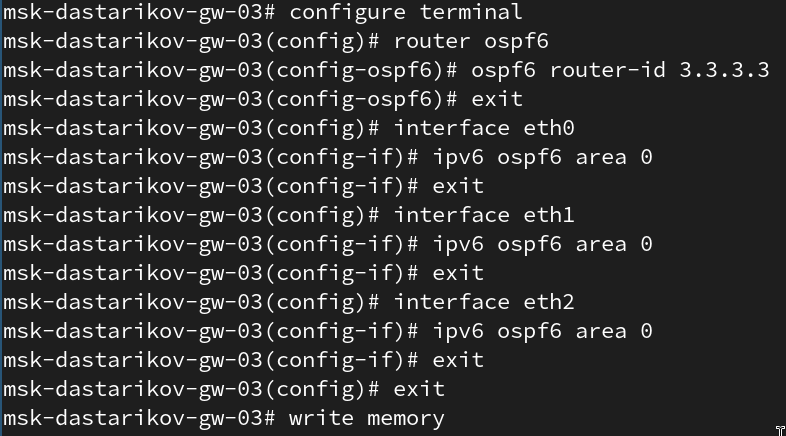
\includegraphics[width=0.8\textwidth]{../images/image55.png}
      \captionof{figure}{Настройка протокола OSPFv3 на маршрутизатору \texttt{gw-03}.}
      \label{55}
    \end{center}

    \begin{center}
      \centering
      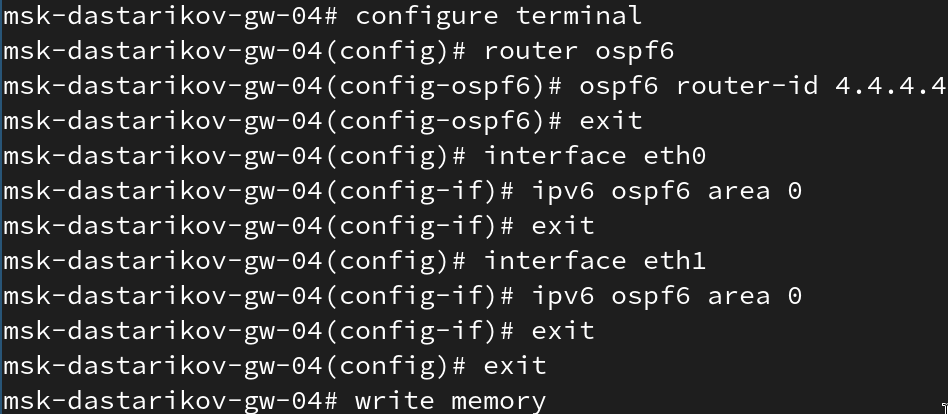
\includegraphics[width=0.8\textwidth]{../images/image56.png}
      \captionof{figure}{Настройка протокола OSPFv3 на маршрутизатору \texttt{gw-04}.}
      \label{56}
    \end{center}

  \item С PC1 пропинговали PC2 и определили путь следования пакетов (рис. \ref{57}):
\begin{minted}{bash}
    PC1> ping 2001:11::a
    PC1> trace 2001:11::a
\end{minted}

    \begin{center}
      \centering
      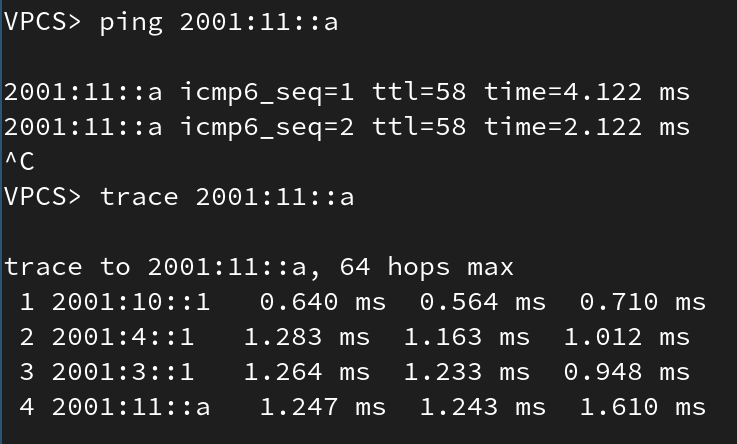
\includegraphics[width=0.8\textwidth]{../images/image57.png}
      \captionof{figure}{Отправка эхо-запроса с PC1 к PC2.}
      \label{57}
    \end{center}

  \item Проверили таблицу маршрутизации протокола OSPFv3 (рис. \ref{58}):
\begin{minted}{bash}
    msk-dastarikov-gw-01# show ipv6 ospf6 neighbor
    msk-dastarikov-gw-01# show ipv6 ospf6 route
\end{minted}

    \begin{center}
      \centering
      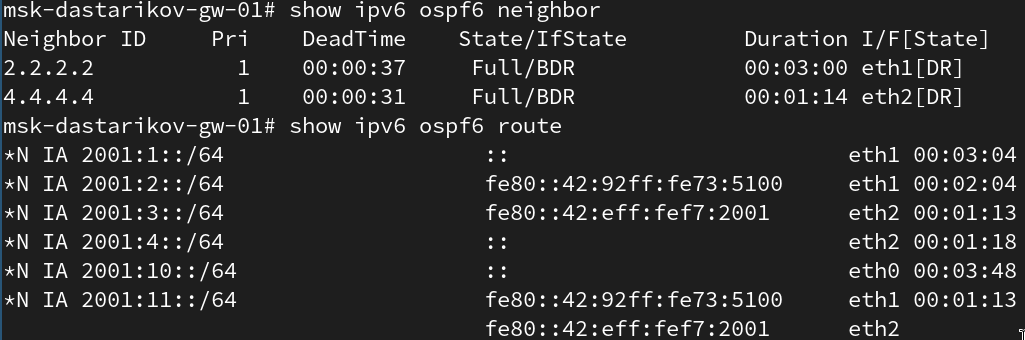
\includegraphics[width=0.8\textwidth]{../images/image58.png}
      \captionof{figure}{Проверка таблицы маршрутизации протокола OSPFv3.}
      \label{58}
    \end{center}


  \item Отключили на маршрутизаторе \texttt{msk-dastarikov-gw-04} интерфейс (рис. \ref{59}):
\begin{minted}{bash}
    msk-dastarikov-gw-04# configure terminal
    msk-dastarikov-gw-04(config)# interface eth0
    msk-dastarikov-gw-04(config-if)# shutdown
\end{minted}

    \begin{center}
      \centering
      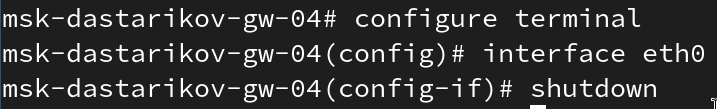
\includegraphics[width=0.8\textwidth]{../images/image59.png}
      \captionof{figure}{Отключение на маршрутизаторе \texttt{msk-dastarikov-gw-04} интерфейса \texttt{eth0}.}
      \label{59}
    \end{center}

  \item Проверили таблицу маршрутизации протокола OSPFv3 (рис. \ref{58}):
\begin{minted}{bash}
    msk-dastarikov-gw-01# show ipv6 ospf6 route
\end{minted}

    \begin{center}
      \centering
      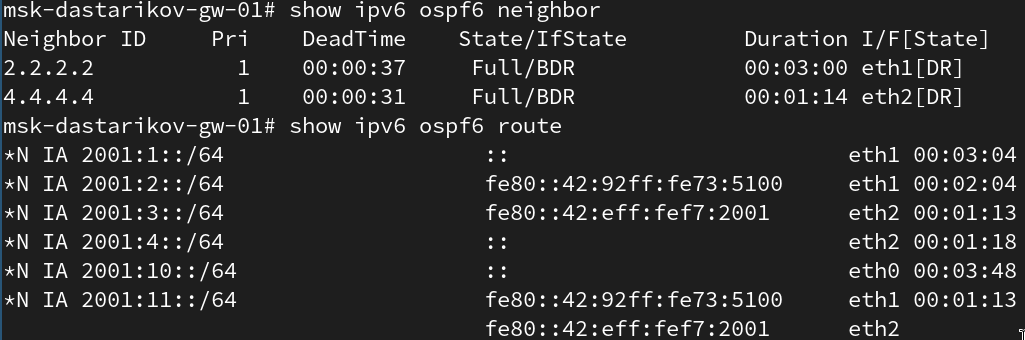
\includegraphics[width=0.8\textwidth]{../images/image58.png}
      \captionof{figure}{Проверка таблицы маршрутизации протокола OSPFv3 после отключения интерфейса маршрутизатора.}
      \label{58}
    \end{center}

  \item С PC1 пропинговали PC2 и определили путь следования пакетов (рис. \ref{61}). Маршрут восстановился почти моментально.

    \begin{center}
      \centering
      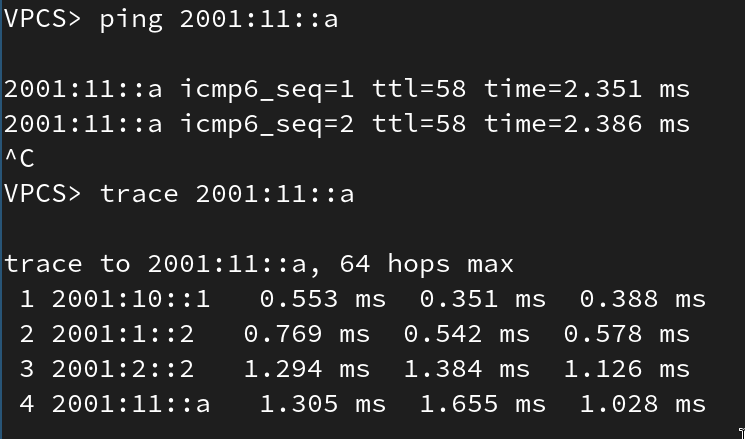
\includegraphics[width=0.8\textwidth]{../images/image61.png}
      \captionof{figure}{Отправка эхо-запроса с PC1 к PC2 по новому маршруту.}
      \label{61}
    \end{center}

  \item Включили на маршрутизаторе \texttt{msk-dastarikov-gw-02} интерфейс:
\begin{minted}{bash}
    msk-dastarikov-gw-02# configure terminal
    msk-dastarikov-gw-02(config)# interface eth0
    msk-dastarikov-gw-02(config-if)# no shutdown
\end{minted}

  \end{enumerate}
  \subsection{Построение туннеля IPv6-IPv4}
  \subsubsection{Постановка задачи}
  Заданы две IPv6-сети и IPv4-сеть (рис. \ref{83}). Требуется организовать туннель IPv6 поверх IPv4, позволяющий передавать данные из одной IPv6-сети в другую IPv6-сеть через сеть IPv4. Назначаемые устройствам сети адреса указаны в табл. \ref{tab3}.

  \begin{table}[]
    \centering
    \caption{Таблица адресации}
    \label{tab3}
    \begin{tabular}{|l|l|l|l|}
      \hline
      Устройство & Интерфейс & Адрес      & Шлюз по умолчанию \\ \hline
      R1         & eth0      & 1000::1/64 & –                 \\ \hline
      R1         & eth1      & 10.0.0.1/8 & –                 \\ \hline
      R1         & Tunnel0   & 1001::1/64 & –                 \\ \hline
      R2         & eth0      & 1002::1/64 & –                 \\ \hline
      R2         & eth1      & 20.0.0.2/8 & –                 \\ \hline
      R2         & Tunnel0   & 1001::2/64 & –                 \\ \hline
      R3         & eth0      & 10.0.0.2/8 & –                 \\ \hline
      R3         & eth1      & 20.0.0.1/8 & –                 \\ \hline
      PC1        & –         & 1000::a/64 & 1000::1           \\ \hline
      PC2        & –         & 1002::a/64 & 1002::1           \\ \hline
    \end{tabular}
  \end{table}

  \begin{center}
    \centering
    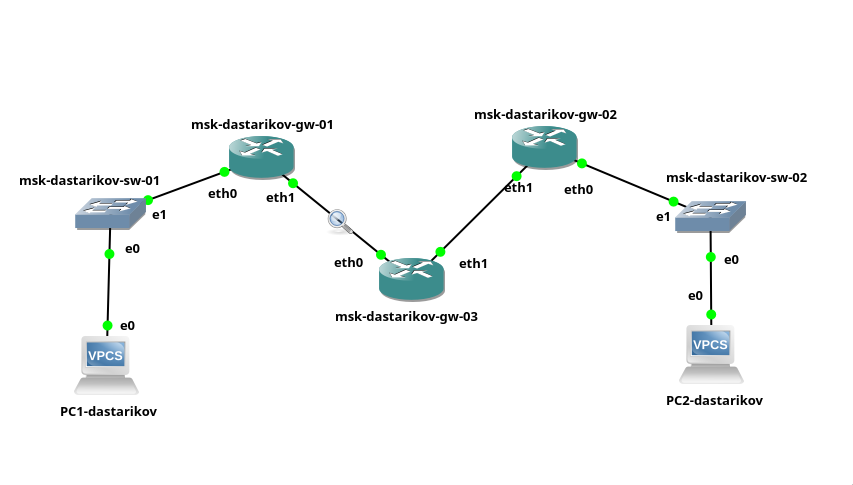
\includegraphics[width=0.8\textwidth]{../images/image83.png}
    \captionof{figure}{Топология сети.}
    \label{83}
  \end{center}

  \subsubsection{Порядок выполнения работы}
  \begin{enumerate}
  \item Создали новый проект в GNS3.
  \item В рабочем пространстве разместили и соединили устройства в соответствии
    с топологией, приведённой на рис. \ref{83}. Использовали маршрутизаторы VyOS.
  \item Изменили отображаемые названия устройств. Коммутаторам присвоили названия по принципу \texttt{msk-dastarikov-sw-0x}, маршрутизаторам — по принципу \texttt{msk-dastarikov-gw-0x}, VPCS — по принципу \texttt{PCx-dastarikov}, где вместо x — порядковый номер устройства.

  \item Присвоили адреса оконечным устройствам PC1 и PC2 в соответствии с данными в табл. \ref{tab3} (рис. \ref{62} и \ref{63}):
\begin{minted}{bash}
    PC1-dastarikov:
    ip 1000::a/64
    save
    show ipv6
\end{minted}
    PC2-dastarikov:
\begin{minted}{bash}
    ip 1002::a/64
    save
    show ipv6
\end{minted}

    \begin{center}
      \centering
      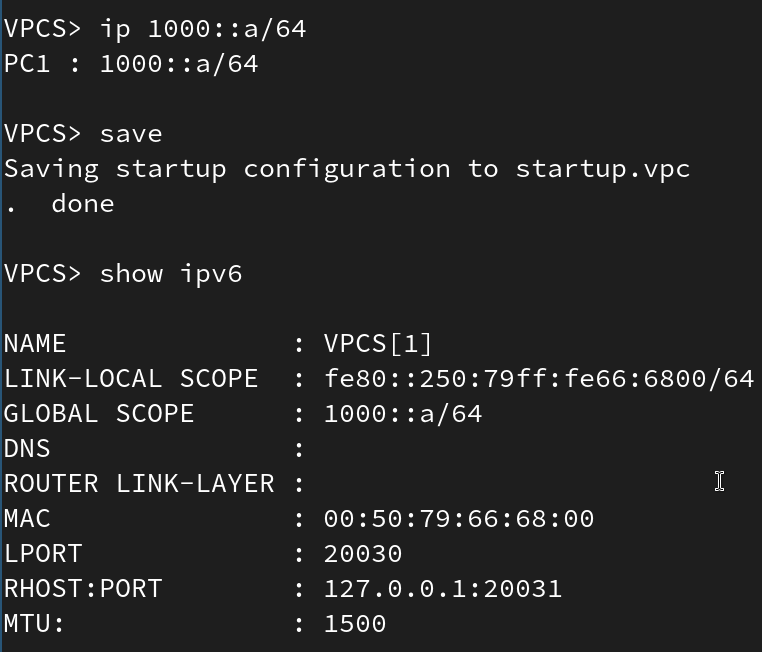
\includegraphics[width=0.8\textwidth]{../images/image62.png}
      \captionof{figure}{Настройка IP-адреса PC1.}
      \label{62}
    \end{center}

    \begin{center}
      \centering
      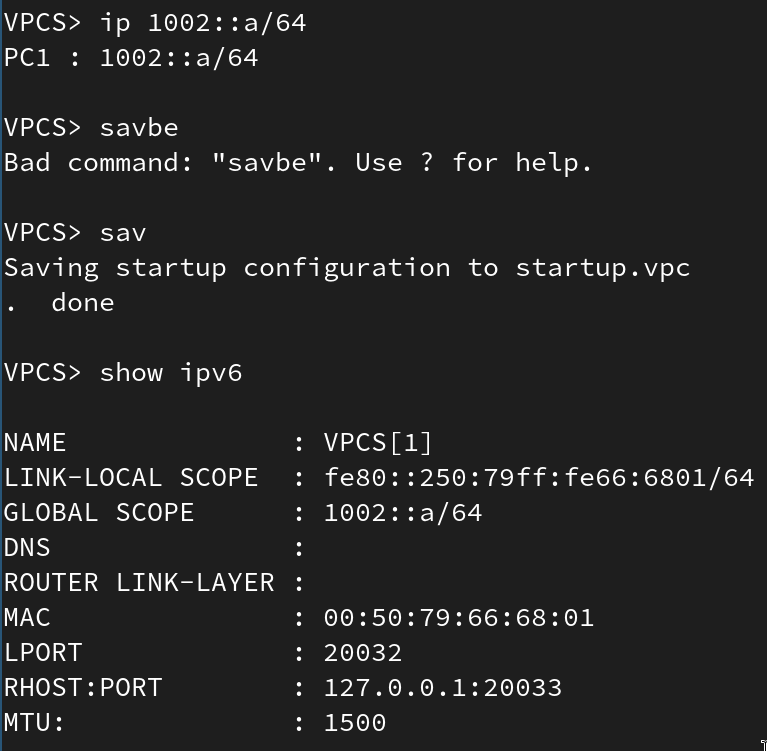
\includegraphics[width=0.8\textwidth]{../images/image63.png}
      \captionof{figure}{Настройка IP-адреса PC2.}
      \label{63}
    \end{center}

  \item Настроили адреса на интерфейсах маршрутизаторов (рис. \ref{64}-\ref{66}):
\begin{minted}{bash}
    msk-dastarikov-gw-01:
    vyos@msk-dastarikov-gw-01:~$ configure
    vyos@msk-dastarikov-gw-01# set interfaces ethernet eth0 address 1000::1/64
    vyos@msk-dastarikov-gw-01# set interfaces ethernet eth1 address 10.0.0.1/8
    vyos@msk-dastarikov-gw-01# set service router-advert interface eth0 prefix 1000::/64
    vyos@msk-dastarikov-gw-01# commit
    vyos@msk-dastarikov-gw-01# save
\end{minted}
    msk-dastarikov-gw-02:
\begin{minted}{bash}
    vyos@msk-dastarikov-gw-02:~$ configure
    vyos@msk-dastarikov-gw-02# set interfaces ethernet eth0 address 1002::1/64
    vyos@msk-dastarikov-gw-02# set interfaces ethernet eth1 address 20.0.0.2/8
    vyos@msk-dastarikov-gw-02# set service router-advert interface eth0 prefix 1002::/64
    vyos@msk-dastarikov-gw-02# commit
    vyos@msk-dastarikov-gw-02# save
\end{minted}
    msk-dastarikov-gw-03:
\begin{minted}{bash}
    vyos@msk-dastarikov-gw-03:~$ configure
    vyos@msk-dastarikov-gw-03# set interfaces ethernet eth0 address 10.0.0.2/8
    vyos@msk-dastarikov-gw-03# set interfaces ethernet eth1 address 20.0.0.1/8
    vyos@msk-dastarikov-gw-03# commit
    vyos@msk-dastarikov-gw-03# save
\end{minted}

    \begin{center}
      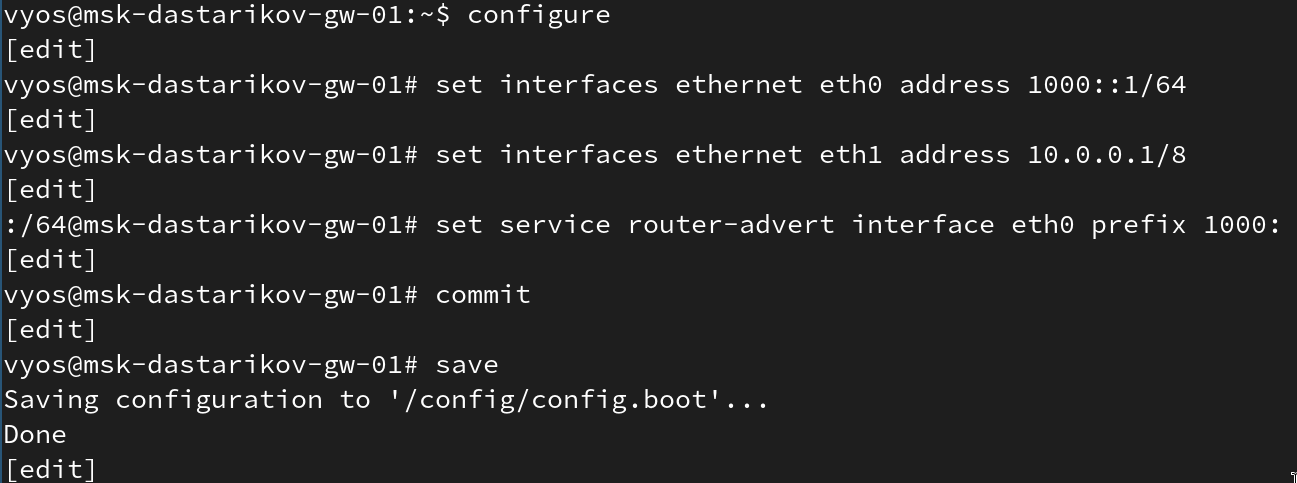
\includegraphics[width=0.8\textwidth]{../images/image64.png}
      \captionof{figure}{Настройка IP-адресации на маршрутизаторе \texttt{gw-01}.}
      \label{64}
    \end{center}

    \begin{center}
      \centering
      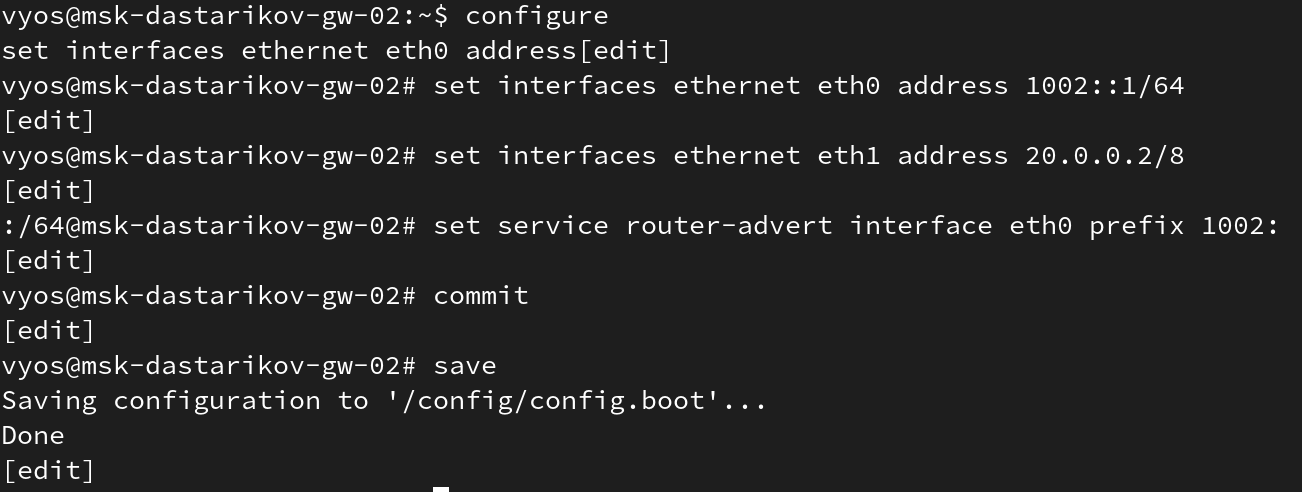
\includegraphics[width=0.8\textwidth]{../images/image65.png}
      \captionof{figure}{Настройка IP-адресации на маршрутизаторе \texttt{gw-02}.}
      \label{65}
    \end{center}

    \begin{center}
      \centering
      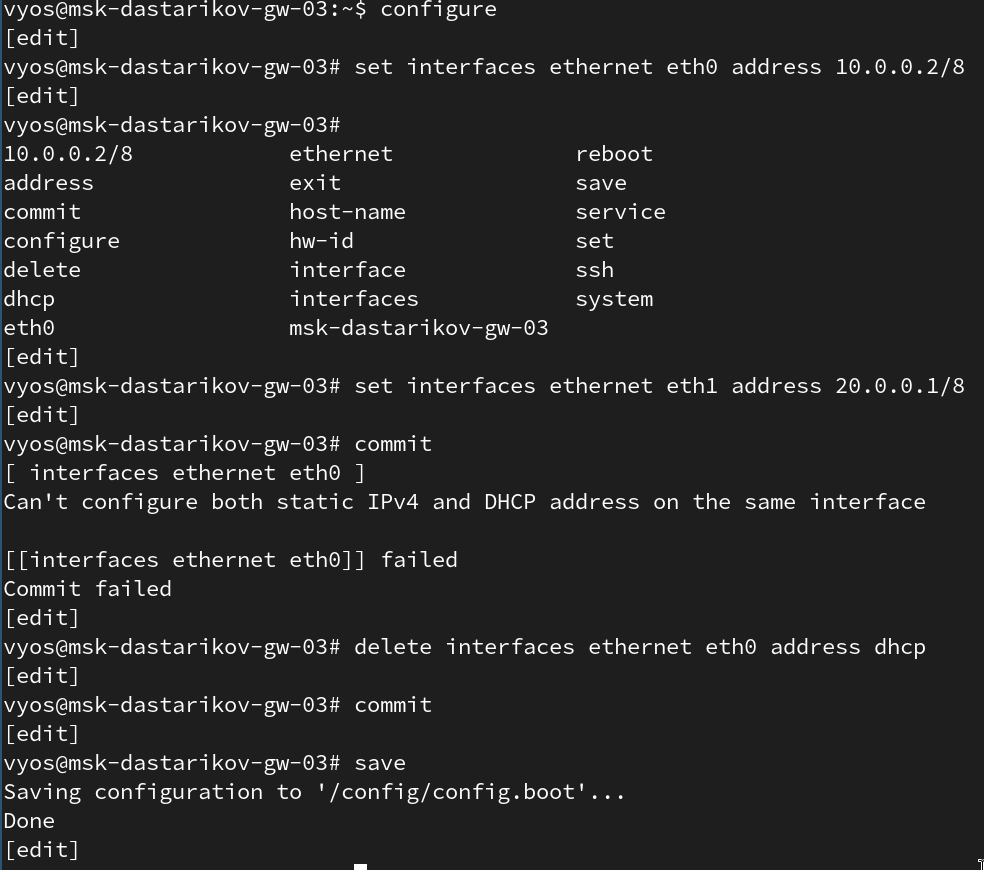
\includegraphics[width=0.8\textwidth]{../images/image66.png}
      \captionof{figure}{Настройка IP-адресации на маршрутизаторе \texttt{gw-03}.}
      \label{66}
    \end{center}

  \item Убедились, что на PC появились адреса ближайших к ним маршрутизаторов (рис. \ref{67} и \ref{68}):
    PC1-dastarikov:
\begin{minted}{bash}
      show ipv6
\end{minted}
    PC2-dastarikov:
\begin{minted}{bash}
      show ipv6
\end{minted}

    \begin{center}
      \centering
      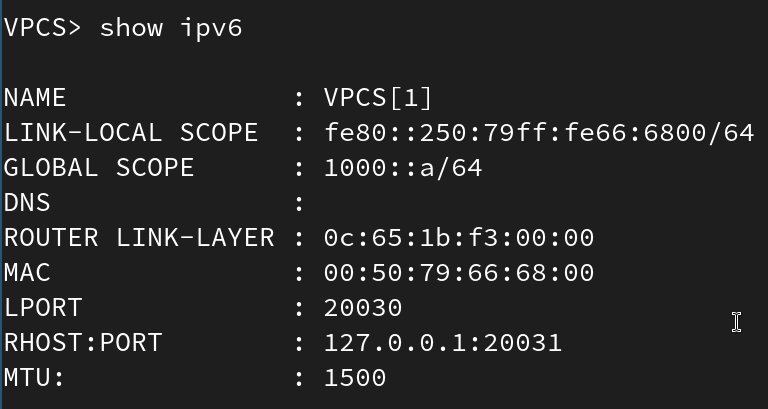
\includegraphics[width=0.8\textwidth]{../images/image67.png}
      \captionof{figure}{Проверка появления адресов ближайщих маршрутизаторов на PC1.}
      \label{67}
    \end{center}

    \begin{center}
      \centering
      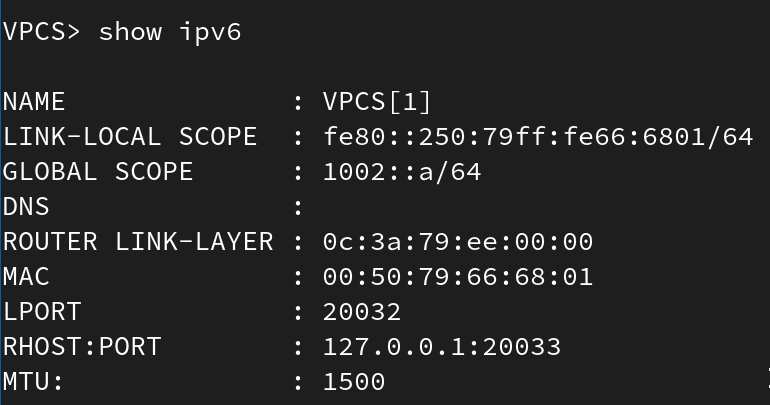
\includegraphics[width=0.8\textwidth]{../images/image68.png}
      \captionof{figure}{Проверка появления адресов ближайщих маршрутизаторов на PC2.}
      \label{68}
    \end{center}

  \item Проверили маршруты с маршрутизатора R1 (рис. \ref{69}):
\begin{minted}{bash}
    vyos@msk-dastarikov-gw-01:~$ ping 10.0.0.2
    vyos@msk-dastarikov-gw-01:~$ ping 20.0.0.1
    vyos@msk-dastarikov-gw-01:~$ ping 20.0.0.2
\end{minted}

    \begin{center}
      \centering
      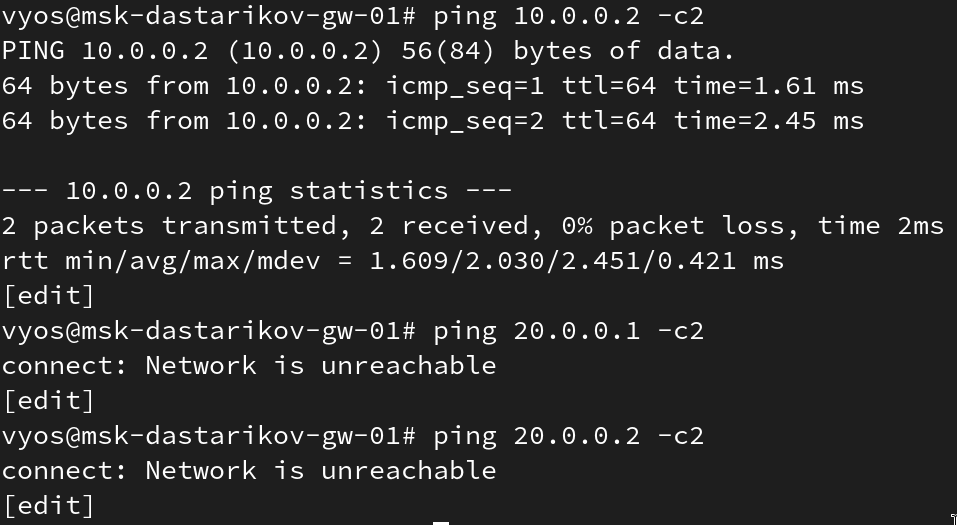
\includegraphics[width=0.8\textwidth]{../images/image69.png}
      \captionof{figure}{Проверка маршрутов с маршрутизатора R1.}
      \label{69}
    \end{center}

    Эхо запросы проходят только до \texttt{10.0.0.2} - адрес интерфейса \texttt{eth0} маршутизатора \texttt{gw-03}, который находится в той же сети. Два остальных адреса не доступны, так как находятся в других подсетях.
    
  \item Настроили маршрутизацию IPv4 (рис. \ref{74}-\ref{76}):
\begin{minted}{bash}
    msk-dastarikov-gw-01:
    vyos@msk-dastarikov-gw-01:~$ configure
    vyos@msk-dastarikov-gw-01# set protocols rip network 10.0.0.0/8
    vyos@msk-dastarikov-gw-01# commit
    vyos@msk-dastarikov-gw-01# save
\end{minted}
    msk-dastarikov-gw-02:
\begin{minted}{bash}
    vyos@msk-dastarikov-gw-02:~$ configure
    vyos@msk-dastarikov-gw-02# set protocols rip network 20.0.0.0/8
    vyos@msk-dastarikov-gw-02# commit
    vyos@msk-dastarikov-gw-02# save
\end{minted}
    msk-dastarikov-gw-03:
\begin{minted}{bash}
    vyos@msk-dastarikov-gw-03:~$ configure
    vyos@msk-dastarikov-gw-03# set protocols rip network 10.0.0.0/8
    vyos@msk-dastarikov-gw-03# set protocols rip network 20.0.0.0/8
    vyos@msk-dastarikov-gw-03# commit
    vyos@msk-dastarikov-gw-03# save
\end{minted}

    \begin{center}
      \centering
      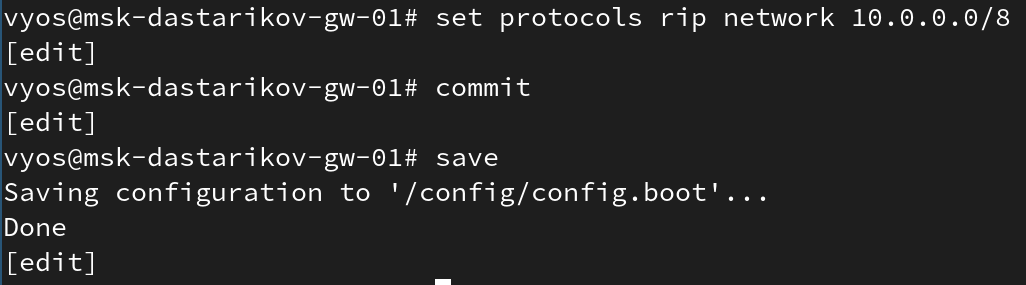
\includegraphics[width=0.8\textwidth]{../images/image74.png}
      \captionof{figure}{Настройка протокола RIP на маршрутизатору \texttt{gw-01}.}
      \label{74}
    \end{center}

    \begin{center}
      \centering
      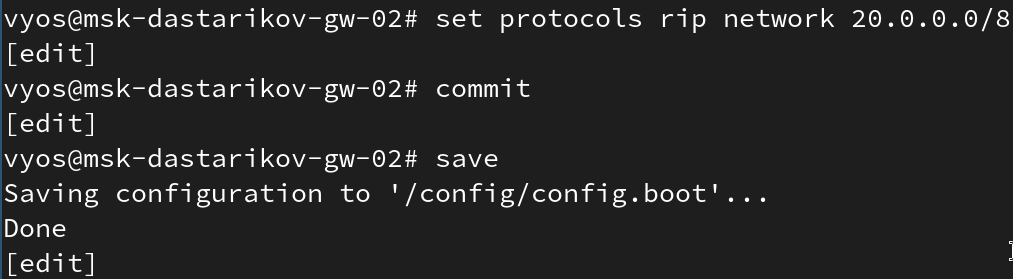
\includegraphics[width=0.8\textwidth]{../images/image75.png}
      \captionof{figure}{Настройка протокола RIP на маршрутизатору \texttt{gw-02}.}
      \label{75}
    \end{center}

    \begin{center}
      \centering
      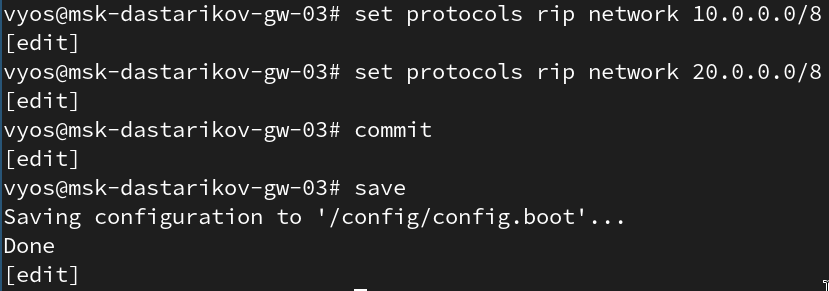
\includegraphics[width=0.8\textwidth]{../images/image76.png}
      \captionof{figure}{Настройка протокола RIP на маршрутизатору \texttt{gw-03}.}
      \label{76}
    \end{center}

  \item Проверили маршруты (рис. \ref{77}):
\begin{minted}{bash}
    vyos@msk-dastarikov-gw-01:~$ ping 10.0.0.2
    vyos@msk-dastarikov-gw-01:~$ ping 20.0.0.1
    vyos@msk-dastarikov-gw-01:~$ ping 20.0.0.2
\end{minted}

    \begin{center}
      \centering
      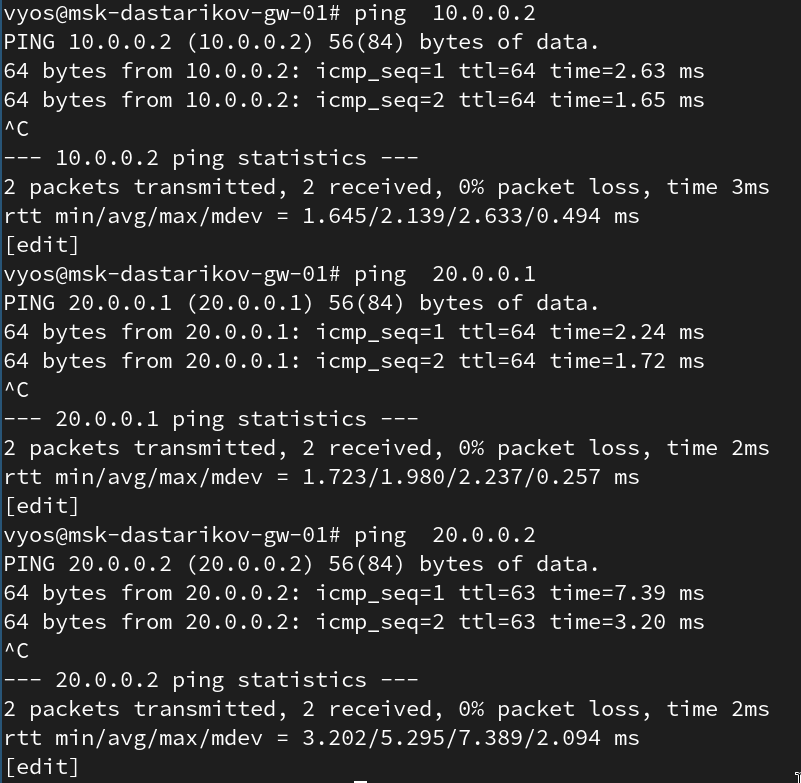
\includegraphics[width=0.8\textwidth]{../images/image77.png}
      \captionof{figure}{Проверка маршрутов с маршрутизатора R1.}
      \label{77}
    \end{center}

    После настройки динамическлой маршрутизации по протоколу RIP эхо-запросы доставляются до всех адресов.

  \item Создали туннель IPv6 через сеть IPv4 (рис. \ref{70} и \ref{71}):
    msk-dastarikov-gw-01:
\begin{minted}{bash}
    vyos@msk-dastarikov-gw-01:~$ configure
    vyos@msk-dastarikov-gw-01# set interfaces tunnel tun0 encapsulation sit
    vyos@msk-dastarikov-gw-01# set interfaces tunnel tun0 source-address 10.0.0.1
    vyos@msk-dastarikov-gw-01# set interfaces tunnel tun0 remote 20.0.0.2
    vyos@msk-dastarikov-gw-01# set interfaces tunnel tun0 address 1001::1/64
    vyos@msk-dastarikov-gw-01# commit
    vyos@msk-dastarikov-gw-01# save
\end{minted}
    msk-dastarikov-gw-02:
\begin{minted}{bash}
    vyos@msk-dastarikov-gw-02:~$ configure
    vyos@msk-dastarikov-gw-02# set interfaces tunnel tun0 encapsulation sit
    vyos@msk-dastarikov-gw-02# set interfaces tunnel tun0 source-address 20.0.0.2
    vyos@msk-dastarikov-gw-02# set interfaces tunnel tun0 remote 10.0.0.1
    vyos@msk-dastarikov-gw-02# set interfaces tunnel tun0 address 1001::2/64
    vyos@msk-dastarikov-gw-02# commit
    vyos@msk-dastarikov-gw-02# save
\end{minted}

    \begin{center}
      \centering
      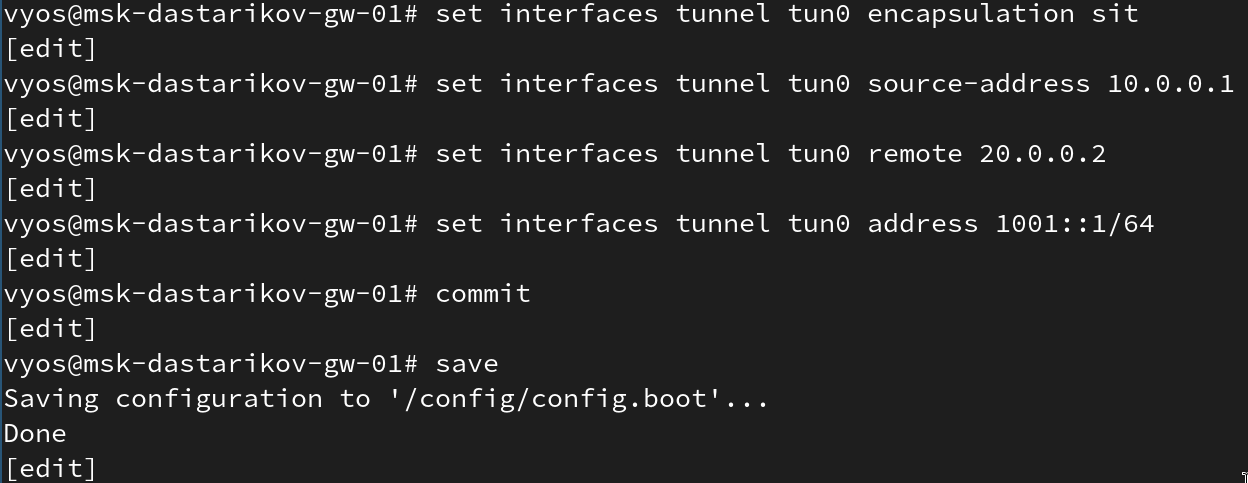
\includegraphics[width=0.8\textwidth]{../images/image70.png}
      \captionof{figure}{Настройка туннеля на маршрутизаторе \texttt{gw-01}.}
      \label{70}
    \end{center}

    \begin{center}
      \centering
      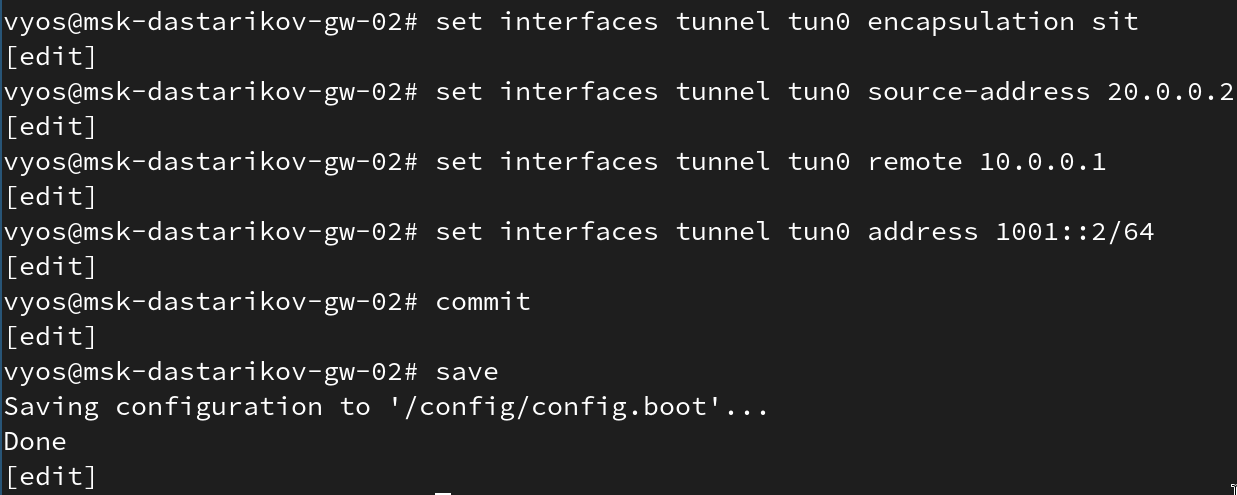
\includegraphics[width=0.8\textwidth]{../images/image71.png}
      \captionof{figure}{Настройка туннеля на маршрутизаторе \texttt{gw-02}.}
      \label{71}
    \end{center}

  \item Настроили статическую маршрутизацию IPv6 (рис. \ref{72} а \ref{73}):
\begin{minted}{bash}
    msk-dastarikov-gw-01:
    vyos@msk-dastarikov-gw-01:~$ configure
    vyos@msk-dastarikov-gw-01# set protocols static route6 1002::0/64 next-hop 1001::2
    vyos@msk-dastarikov-gw-01# commit
    vyos@msk-dastarikov-gw-01# save
\end{minted}
    msk-dastarikov-gw-02:
\begin{minted}{bash}
    vyos@msk-dastarikov-gw-02:~$ configure
    vyos@msk-dastarikov-gw-02# set protocols static route6 1000::0/64 next-hop 1001::1
    vyos@msk-dastarikov-gw-02# commit
    vyos@msk-dastarikov-gw-02# save
\end{minted}


    \begin{center}
      \centering
      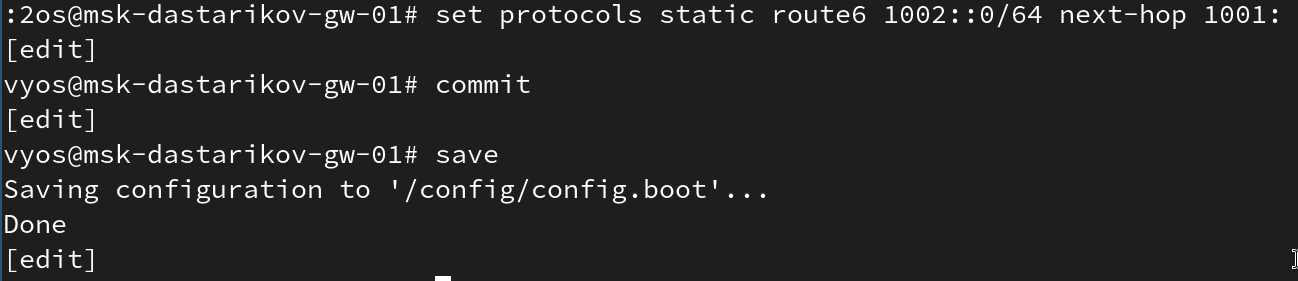
\includegraphics[width=0.8\textwidth]{../images/image72.png}
      \captionof{figure}{Настройка статической маршрутизации IPv6 на маршрутизаторе \texttt{gw-01}.}
      \label{72}
    \end{center}

    \begin{center}
      \centering
      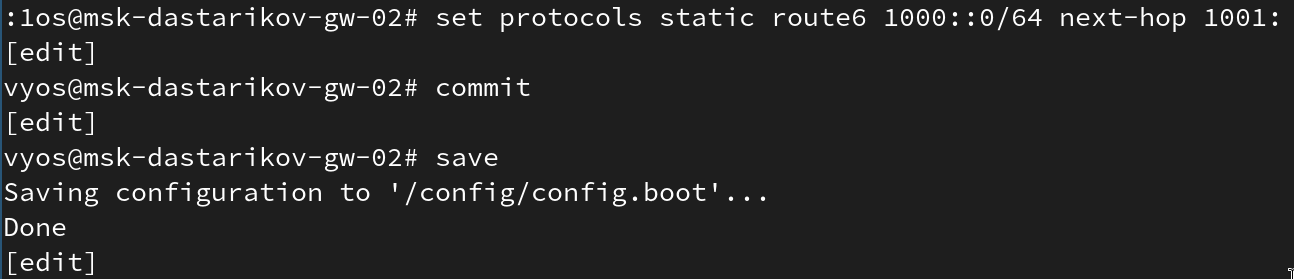
\includegraphics[width=0.8\textwidth]{../images/image73.png}
      \captionof{figure}{Настройка статической маршрутизации IPv6 на маршрутизаторе \texttt{gw-02}.}
      \label{73}
    \end{center}

  \item Проверили доступность оконечных устройств (рис. \ref{79} и \ref{80}):
\begin{minted}{bash}
    PC1-dastarikov:
    PC1-dastarikov> ping 1002::a
    PC1-dastarikov> trace 1002::a
\end{minted}
    PC2-dastarikov:
\begin{minted}{bash}
    PC2-dastarikov> ping 1000::a
    PC2-dastarikov> trace 1000::a
\end{minted}


    \begin{center}
      \centering
      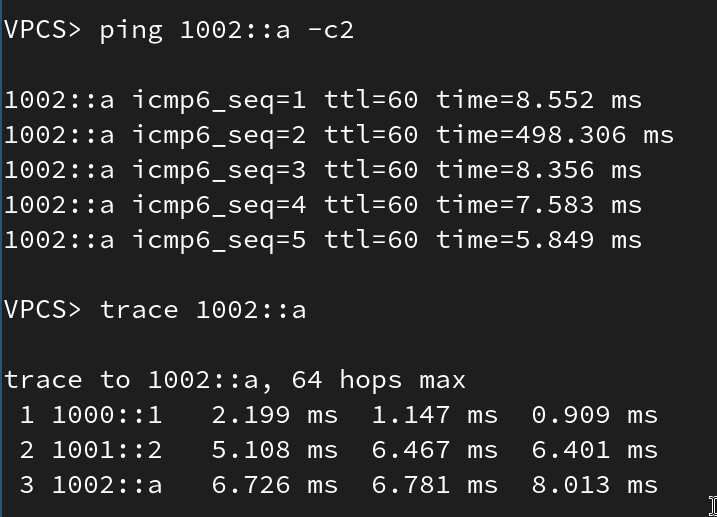
\includegraphics[width=0.8\textwidth]{../images/image79.png}
      \captionof{figure}{Проверка доступности PC2 с PC1.}
      \label{79}
    \end{center}

    \begin{center}
      \centering
      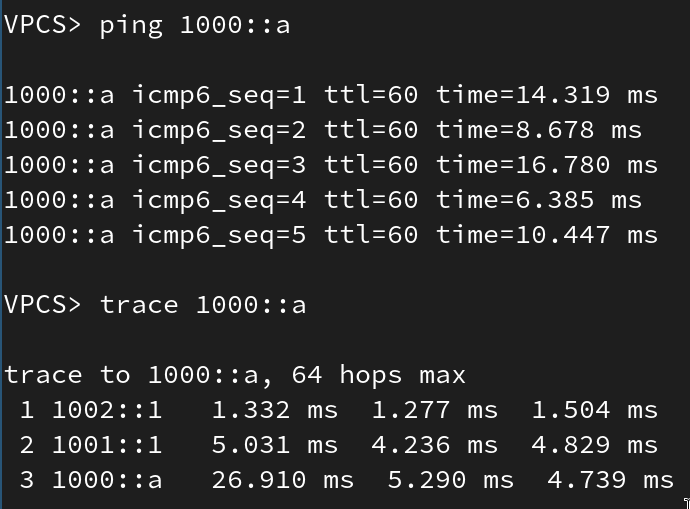
\includegraphics[width=0.8\textwidth]{../images/image80.png}
      \captionof{figure}{Проверка доступности PC1 с PC2.}
      \label{80}
    \end{center}

    Пакеты, проходящие по туннелю, имеют одновременно поля IPv4 и IPv6 (рис. \ref{81} и \ref{82}):

    \begin{center}
      \centering
      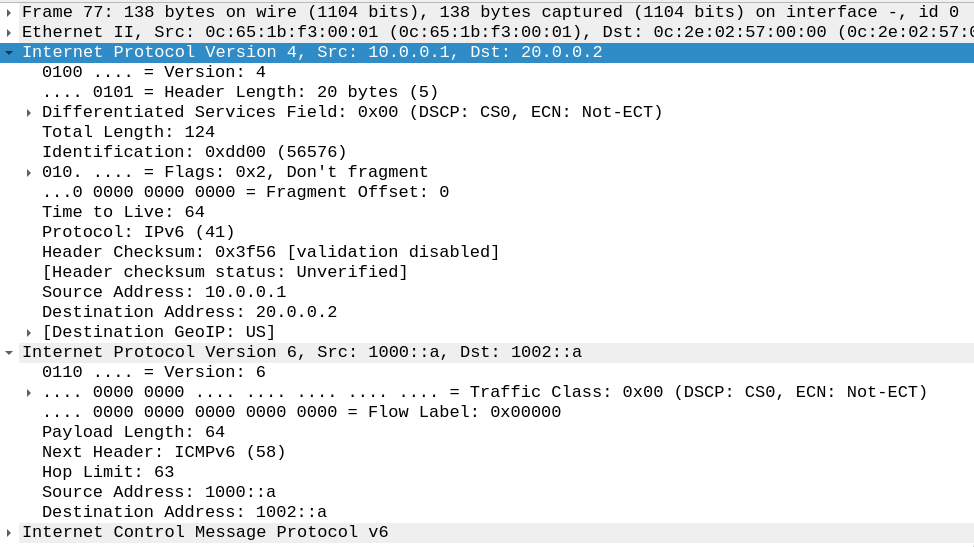
\includegraphics[width=0.8\textwidth]{../images/image81.png}
      \captionof{figure}{Перехваченый эхо-запрос с PC1 к PC2.}
      \label{81}
    \end{center}

    \begin{center}
      \centering
      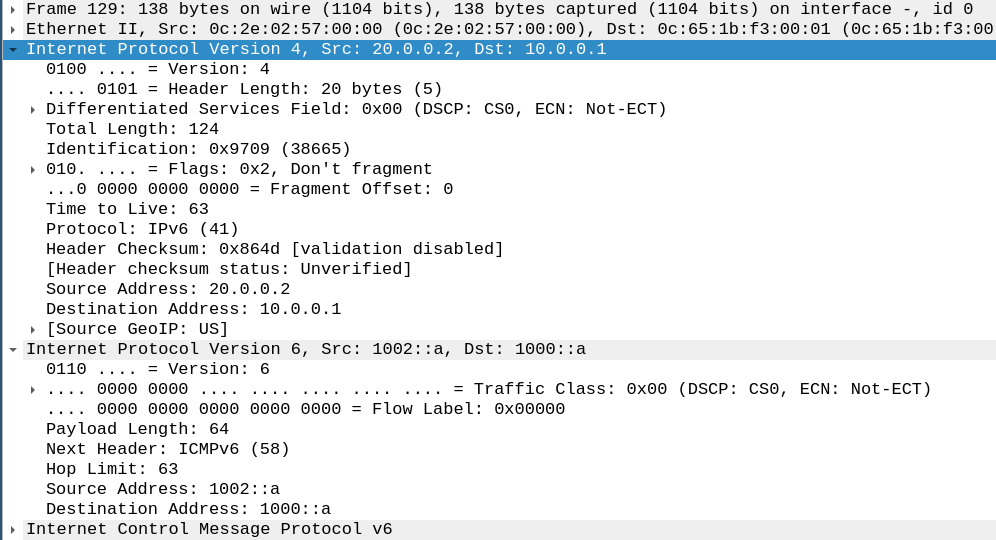
\includegraphics[width=0.8\textwidth]{../images/image82.png}
      \captionof{figure}{Перехваченый эхо-запрос с PC2 к PC1.}
      \label{82}
    \end{center}


  \end{enumerate}
  \subsection{Задание для самостоятельного выполнения}
  Заданы топология сети (рис. \ref{133}) и адреса сегментов сети (табл. \ref{tab6}).

  \begin{center}
    \centering
    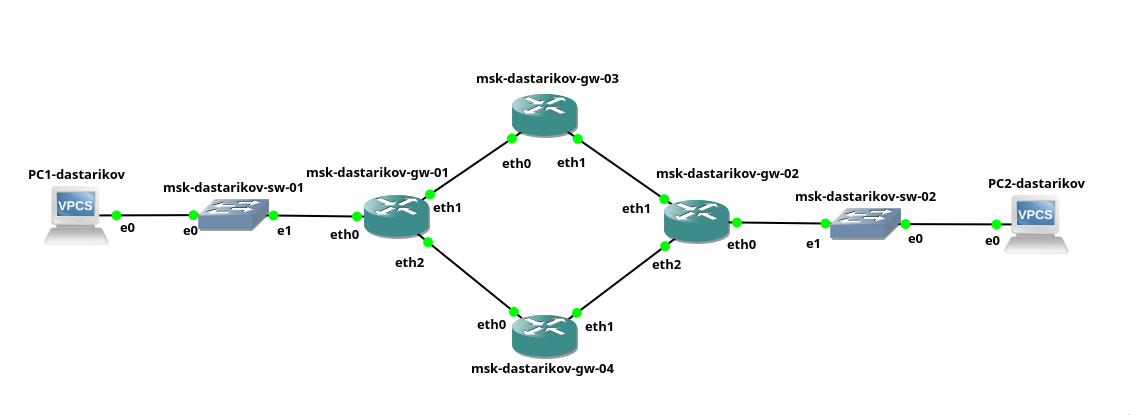
\includegraphics[width=0.8\textwidth]{../images/image133.png}
    \captionof{figure}{Топология сети.}
    \label{133}
  \end{center}

  \begin{table}[]
    \centering
    \caption{Таблица адресов сетей}
    \label{tab6}
    \begin{tabular}{lll}
      Устройства  & Сеть IPv4     & Сеть IPv6         \\
      PC1–gw-01   & 10.10.1.96/27 & 2001:db8:1:1::/64 \\
      PC2–gw-02   & 10.10.1.64/28 & 2001:db8:1:6::/64 \\
      gw-01–gw-03 & 10.10.1.4/30  & 2001:db8:1:2::/64 \\
      gw-02–gw-04 & 10.10.1.8/30  & 2001:db8:1:3::/64 \\
      gw-03–gw-02 & 10.10.1.16/30 & 2001:db8:1:4::/64 \\
      gw-04–gw-02 & 10.10.1.32/30 & 2001:db8:1:5::/64
    \end{tabular}
  \end{table}

  Требуется:
  \begin{enumerate}
  \item настроить двойной стек IPv4 и IPv6, проверить соединения;
  \item настроить динамическую маршрутизацию сетей IPv4 и IPv6 для протоколов RIP, OSPF, проверить соединения и маршруты.
  \end{enumerate}

  \subsubsection{Выполнение}
  \begin{enumerate}
  \item Составили таблицу адресации (табл. \ref{tab4}):
    \begin{table}[]
      \centering
      \caption{Таблица адресации}
      \label{tab4}
      \begin{tabular}{|l|l|l|l|l|}
        \hline
        Устройство           & Интерфейс & Адрес              & Шлюз по умолчанию & След. устройство \\ \hline
        PC1-dastarikov       & NIC       & 10.10.1.98/27      & 10.10.1.97        & gw-01                \\ 
        PC1-dastarikov       & NIC       & 2001:db8:1:1::2/64 & n/a               & gw-01                \\ \hline
        PC2-dastarikov       & NIC       & 10.10.1.66/28      & 10.10.1.65        & gw-02                \\ 
        PC2-dastarikov       & NIC       & 2001:db8:1:6::2/64 & n/a               & gw-02                \\ \hline
        msk-dastarikov-gw-01 & eth0      & 10.10.1.97/27      & n/a               & PC1                  \\ 
        msk-dastarikov-gw-01 & eth0      & 2001:db8:1:1::1/64 & n/a               & PC1                  \\ 
        msk-dastarikov-gw-01 & eth1      & 10.10.1.5/30       & n/a               & gw-03                \\ 
        msk-dastarikov-gw-01 & eth1      & 2001:db8:1:2::1/64 & n/a               & gw-03                \\ 
        msk-dastarikov-gw-01 & eth2      & 10.10.1.9/30       & n/a               & gw-04                \\ 
        msk-dastarikov-gw-01 & eth2      & 2001:db8:1:3::1/64 & n/a               & gw-04                \\ \hline
        msk-dastarikov-gw-02 & eth0      & 10.10.1.65/28      & n/a               & PC2                  \\ 
        msk-dastarikov-gw-02 & eth0      & 2001:db8:1:6::1/64 & n/a               & PC2                  \\ 
        msk-dastarikov-gw-02 & eth1      & 10.10.1.18/30      & n/a               & gw-03                \\ 
        msk-dastarikov-gw-02 & eth1      & 2001:db8:1:4::1/64 & n/a               & gw-03                \\ 
        msk-dastarikov-gw-02 & eth2      & 10.10.1.33/30      & n/a               & gw-04                \\ 
        msk-dastarikov-gw-02 & eth2      & 2001:db8:1:5::1/64 & n/a               & gw-04                \\ \hline
        msk-dastarikov-gw-03 & eth0      & 10.10.1.6/30       & n/a               & gw-01                \\ 
        msk-dastarikov-gw-03 & eth0      & 2001:db8:1:2::2/64 & n/a               & gw-01                \\ 
        msk-dastarikov-gw-03 & eth1      & 10.10.1.17/30      & n/a               & gw-02                \\ 
        msk-dastarikov-gw-03 & eth1      & 2001:db8:1:4::2/64 & n/a               & gw-02                \\ \hline
        msk-dastarikov-gw-04 & eth0      & 10.10.1.10/30      & n/a               & gw-01                \\ 
        msk-dastarikov-gw-04 & eth0      & 2001:db8:1:3::2/64 & n/a               & gw-01                \\ 
        msk-dastarikov-gw-04 & eth1      & 10.10.1.34/30      & n/a               & gw-02                \\ 
        msk-dastarikov-gw-04 & eth1      & 2001:db8:1:5::2/64 & n/a               & gw-02                \\ \hline
      \end{tabular}
    \end{table}

  \item Задали IP-адреса для \texttt{PC1-dastarikov} и \texttt{PC2-dastarikov} (рис. \ref{84} и \ref{85}):

    \begin{center}
      \centering
      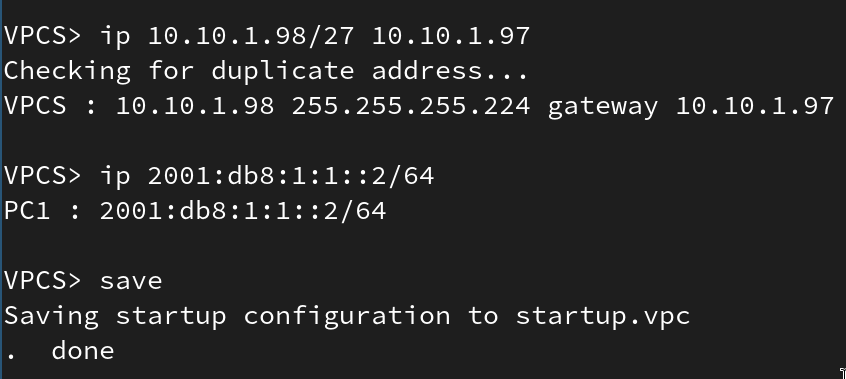
\includegraphics[width=0.8\textwidth]{../images/image84.png}
      \captionof{figure}{Настройка IP-адреса PC1.}
      \label{84}
    \end{center}

    \begin{center}
      \centering
      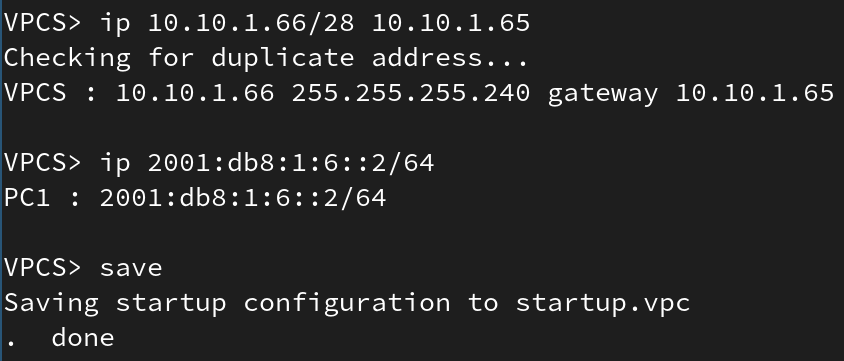
\includegraphics[width=0.8\textwidth]{../images/image85.png}
      \captionof{figure}{Настройка IP-адреса PC2.}
      \label{85}
    \end{center}

  \item Настроили статические IPv4-адреса на маршрутизаторах (рис. \ref{86}-\ref{90}):

    \begin{center}
      \centering
      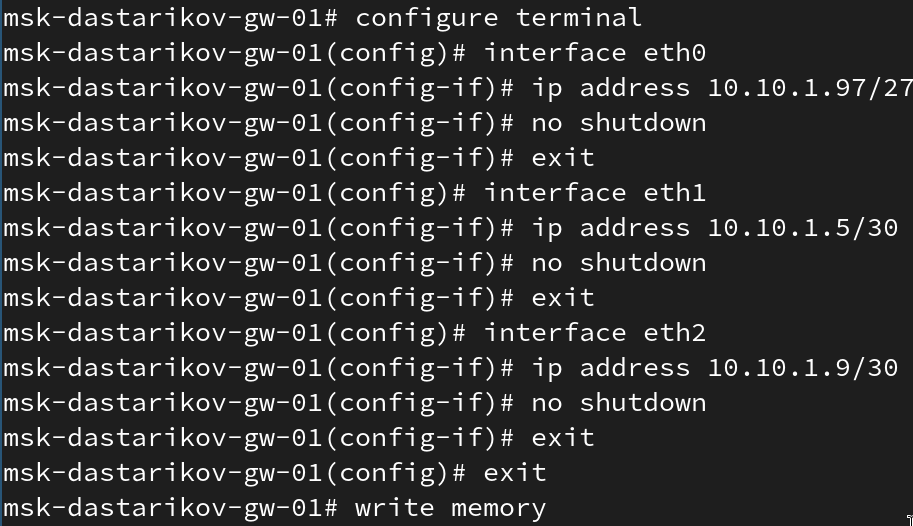
\includegraphics[width=0.8\textwidth]{../images/image86.png}
      \captionof{figure}{Настройка IPv4-адресации на маршрутизаторе \texttt{gw-01}.}
      \label{86}
    \end{center}

    \begin{center}
      \centering
      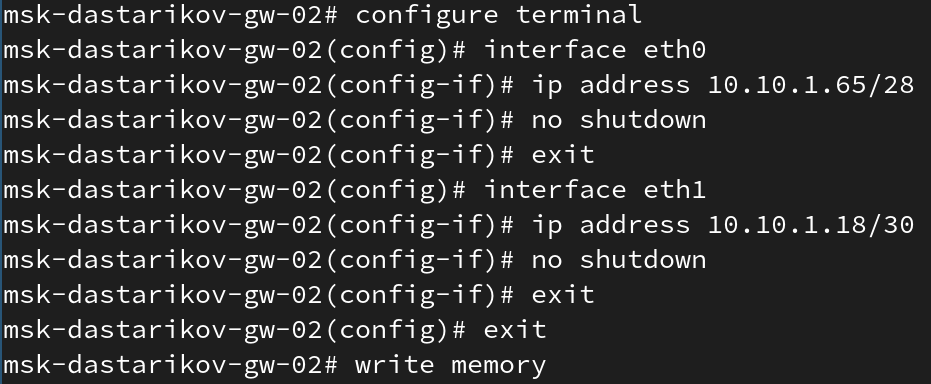
\includegraphics[width=0.8\textwidth]{../images/image87.png}
      \captionof{figure}{Настройка IPv4-адресации на маршрутизаторе \texttt{gw-02} (Часть 1).}
      \label{87}
    \end{center}

    \begin{center}
      \centering
      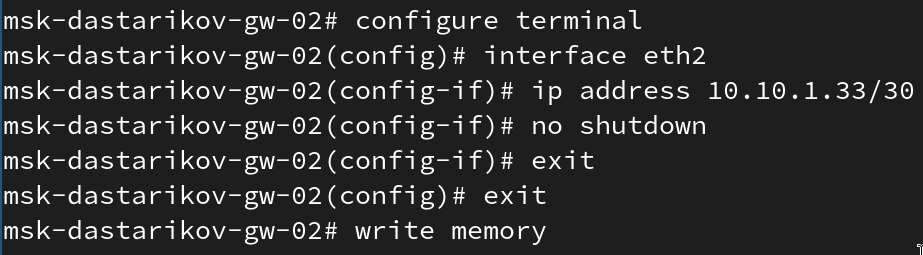
\includegraphics[width=0.8\textwidth]{../images/image88.png}
      \captionof{figure}{Настройка IPv4-адресации на маршрутизаторе \texttt{gw-02} (Часть 2).}
      \label{88}
    \end{center}

    \begin{center}
      \centering
      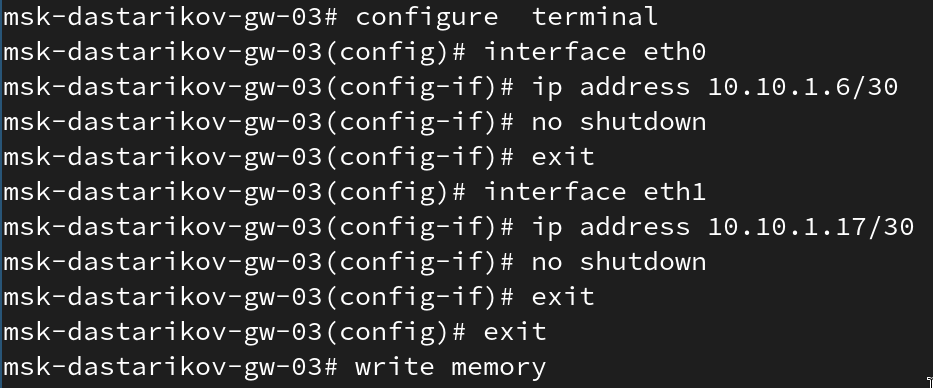
\includegraphics[width=0.8\textwidth]{../images/image89.png}
      \captionof{figure}{Настройка IPv4-адресации на маршрутизаторе \texttt{gw-03}.}
      \label{89}
    \end{center}
    
    \begin{center}
      \centering
      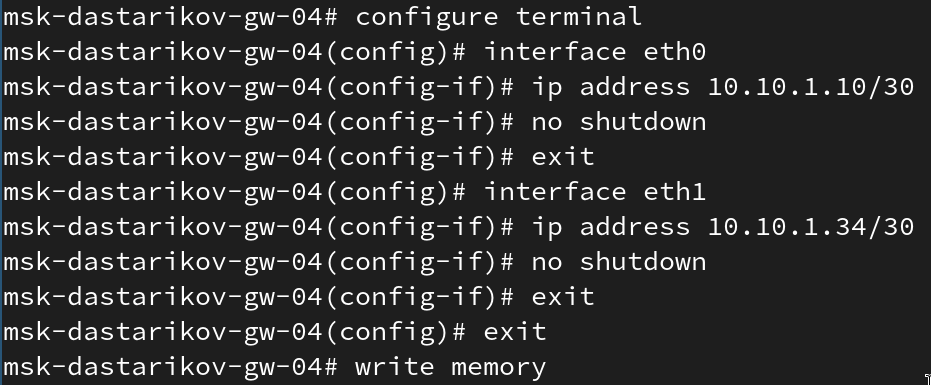
\includegraphics[width=0.8\textwidth]{../images/image90.png}
      \captionof{figure}{Настройка IPv4-адресации на маршрутизаторе \texttt{gw-04}.}
      \label{90}
    \end{center}

  \item Настроили статические IPv6-адреса на маршрутизаторах (рис. \ref{91}-\ref{94}):

    \begin{center}
      \centering
      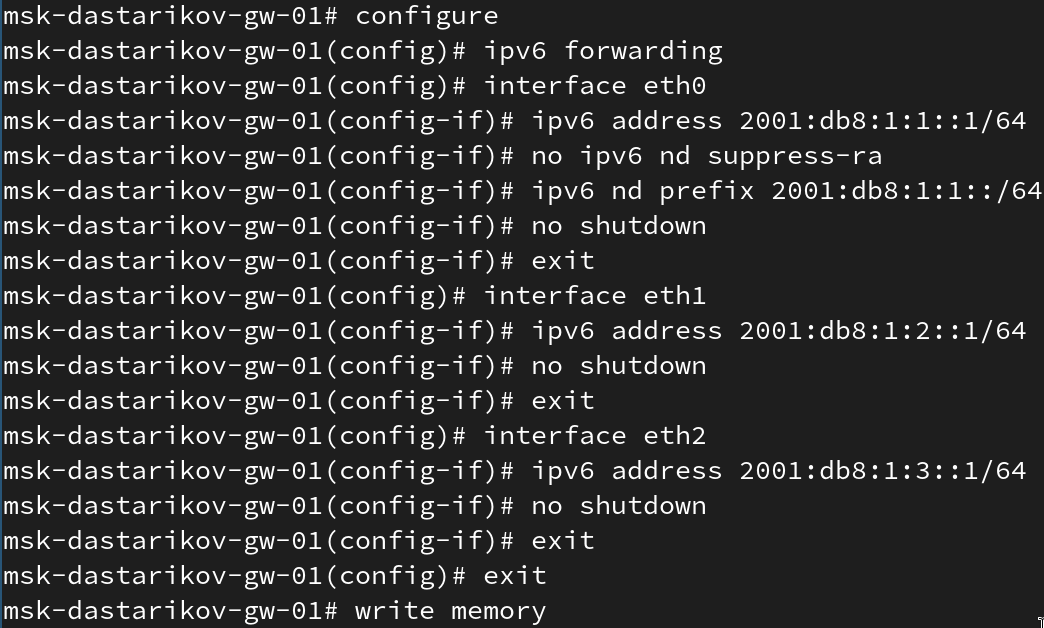
\includegraphics[width=0.8\textwidth]{../images/image91.png}
      \captionof{figure}{Настройка IPv4-адресации на маршрутизаторе \texttt{gw-01}.}
      \label{91}
    \end{center}

    \begin{center}
      \centering
      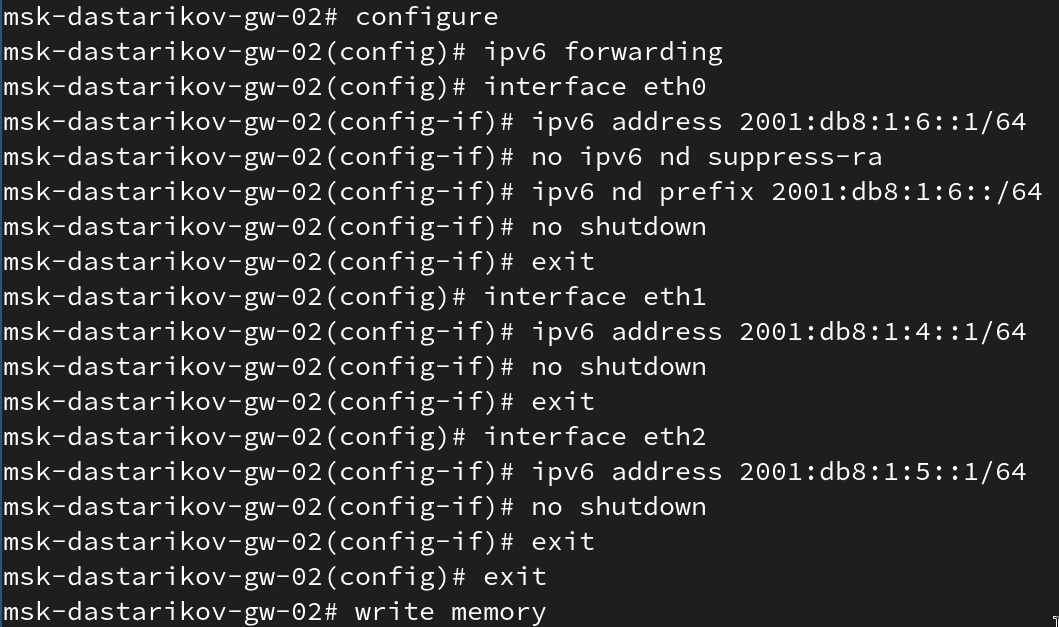
\includegraphics[width=0.8\textwidth]{../images/image92.png}
      \captionof{figure}{Настройка IPv4-адресации на маршрутизаторе \texttt{gw-02}.}
      \label{92}
    \end{center}

    \begin{center}
      \centering
      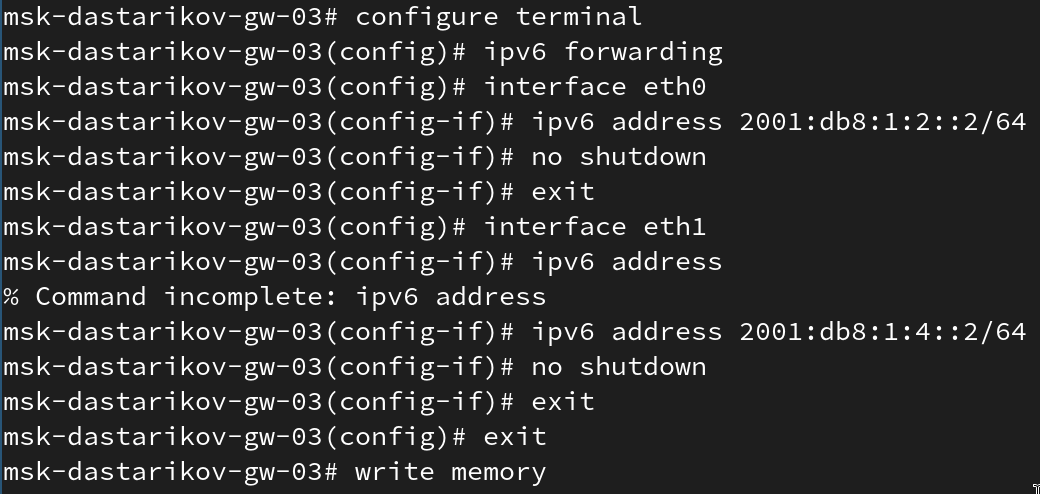
\includegraphics[width=0.8\textwidth]{../images/image93.png}
      \captionof{figure}{Настройка IPv4-адресации на маршрутизаторе \texttt{gw-03}.}
      \label{93}
    \end{center}

    \begin{center}
      \centering
      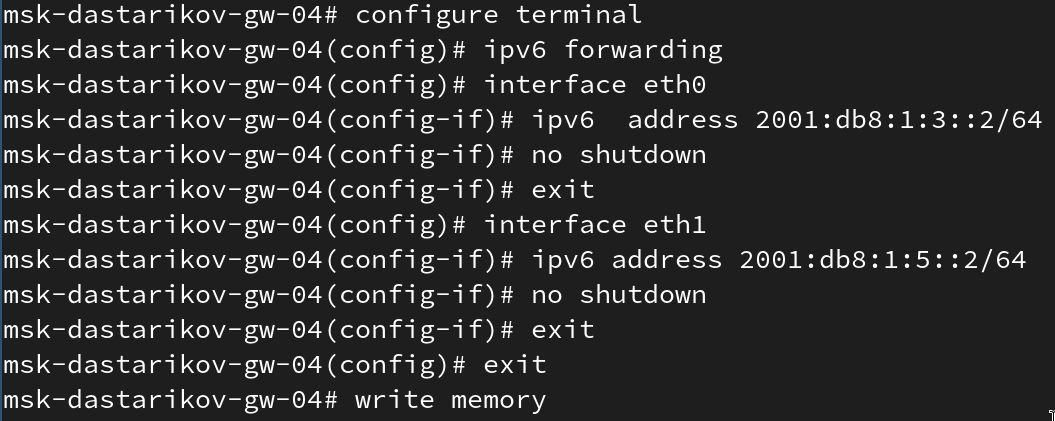
\includegraphics[width=0.8\textwidth]{../images/image94.png}
      \captionof{figure}{Настройка IPv4-адресации на маршрутизаторе \texttt{gw-04}.}
      \label{94}
    \end{center}

  \item Настроили динамическую маршрутизацию по протоколу RIP (рис. \ref{95}-\ref{98}):

    \begin{center}
      \centering
      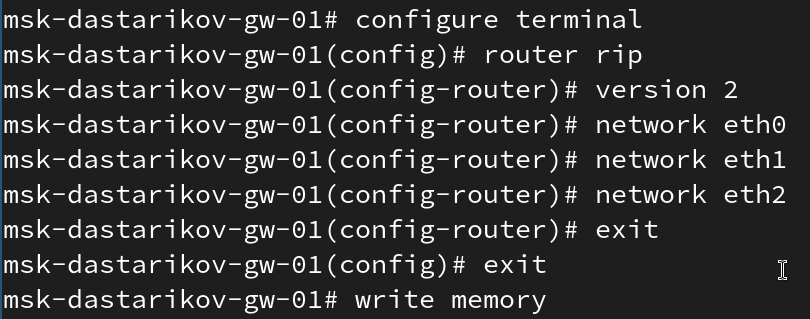
\includegraphics[width=0.8\textwidth]{../images/image95.png}
      \captionof{figure}{Настройка протокола RIP на маршрутизатору \texttt{gw-01}.}
      \label{95}
    \end{center}

    \begin{center}
      \centering
      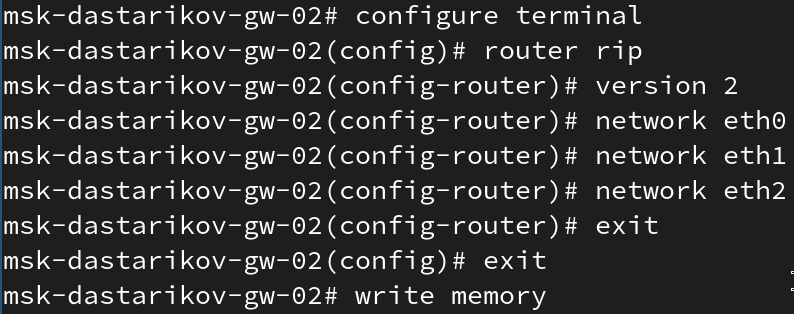
\includegraphics[width=0.8\textwidth]{../images/image96.png}
      \captionof{figure}{Настройка протокола RIP на маршрутизатору \texttt{gw-02}.}
      \label{96}
    \end{center}

    \begin{center}
      \centering
      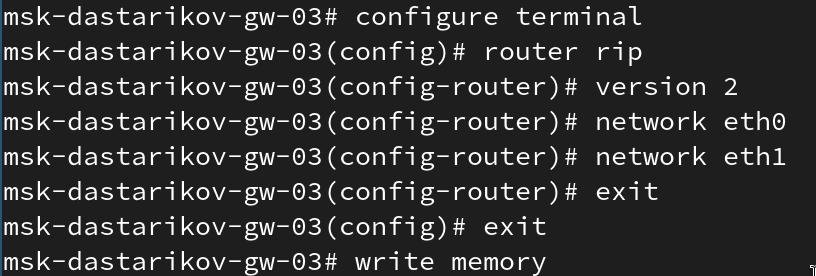
\includegraphics[width=0.8\textwidth]{../images/image97.png}
      \captionof{figure}{Настройка протокола RIP на маршрутизатору \texttt{gw-03}.}
      \label{97}
    \end{center}

    \begin{center}
      \centering
      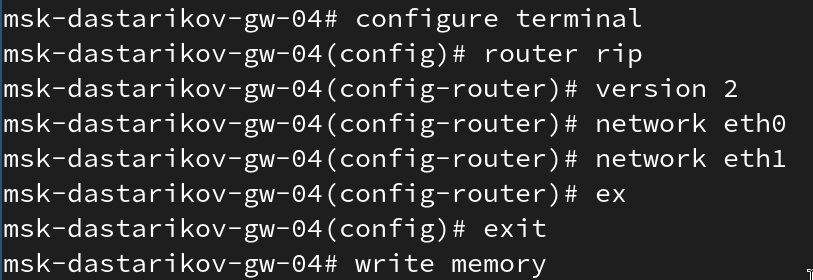
\includegraphics[width=0.8\textwidth]{../images/image98.png}
      \captionof{figure}{Настройка протокола RIP на маршрутизатору \texttt{gw-04}.}
      \label{98}
    \end{center}

  \item Убедились, что маршрутизация по RIP настроена (рис. \ref{99}-\ref{101}):

    \begin{center}
      \centering
      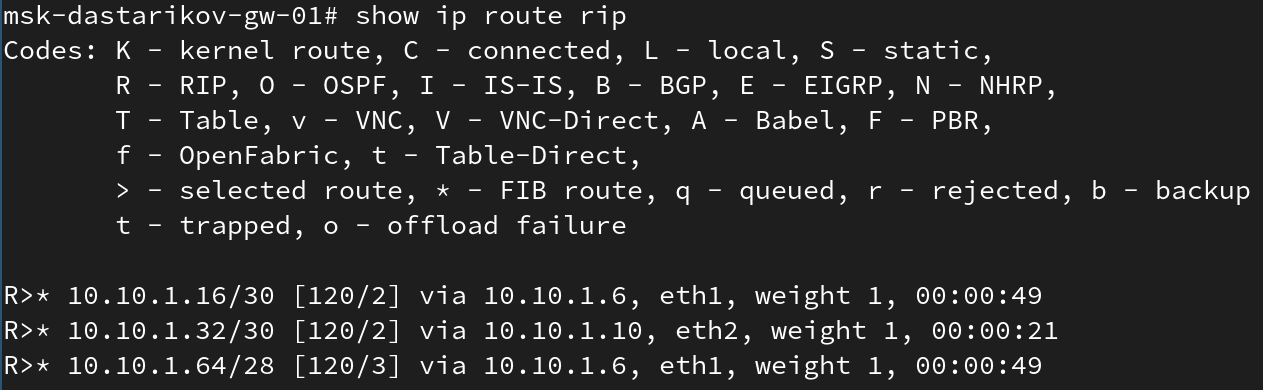
\includegraphics[width=0.8\textwidth]{../images/image99.png}
      \captionof{figure}{Просмотр настроек маршрутизации по RIP.}
      \label{99}
    \end{center}

    \begin{center}
      \centering
      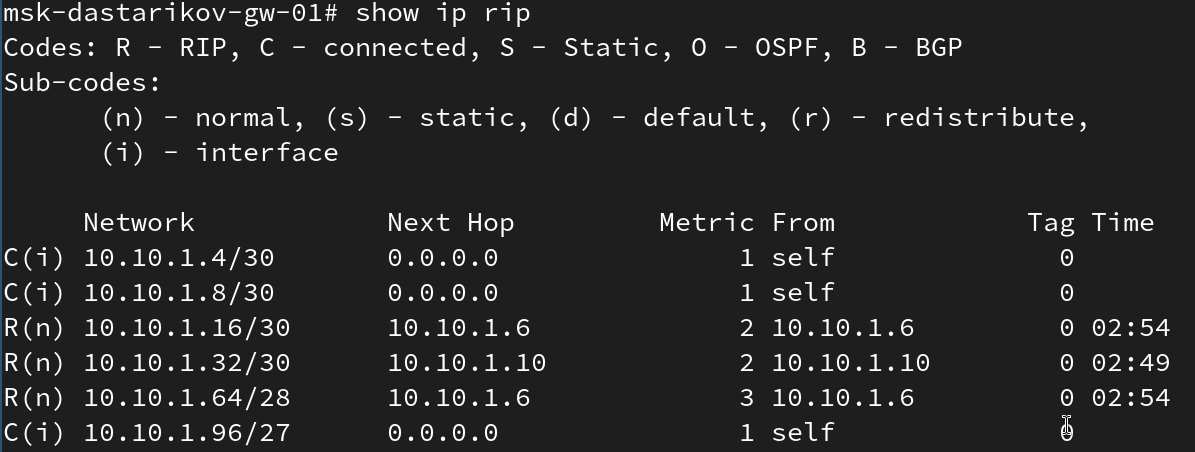
\includegraphics[width=0.8\textwidth]{../images/image100.png}
      \captionof{figure}{Просмотр настроек маршрутизации по RIP.}
      \label{100}
    \end{center}

    \begin{center}
      \centering
      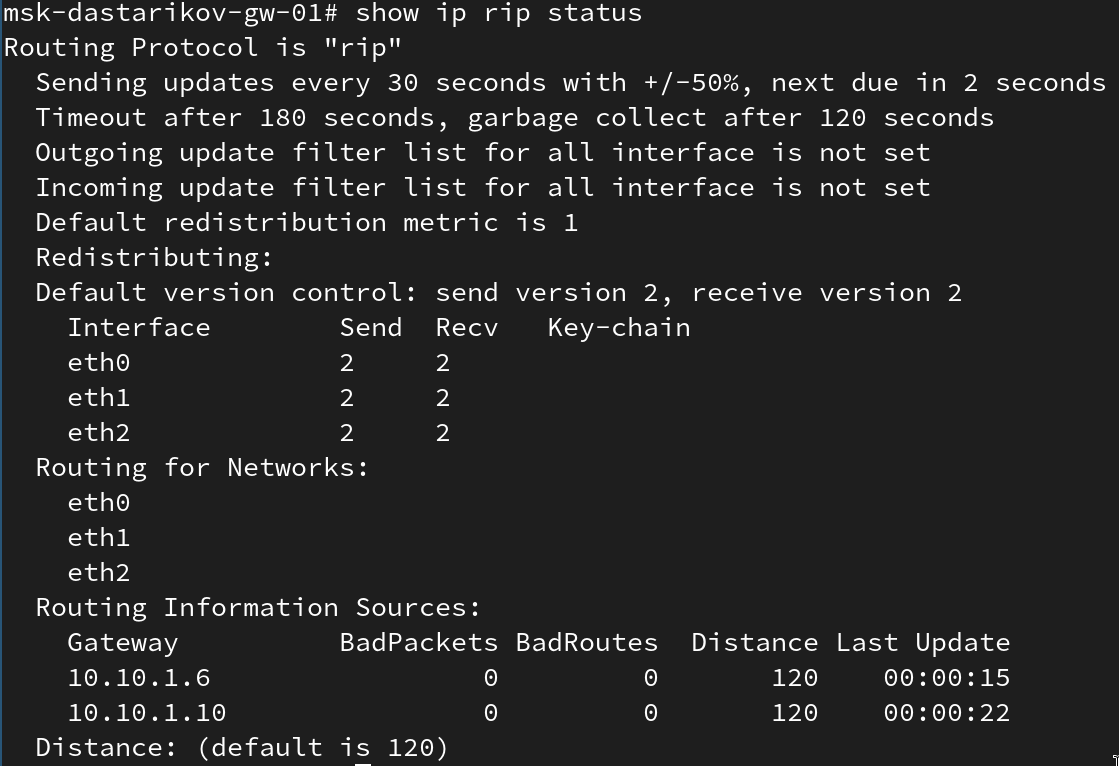
\includegraphics[width=0.8\textwidth]{../images/image101.png}
      \captionof{figure}{Просмотр настроек маршрутизации по RIP.}
      \label{101}
    \end{center}

  \item Проверили доступность оконечных устройств (рис. \ref{102} и \ref{103}):


    \begin{center}
      \centering
      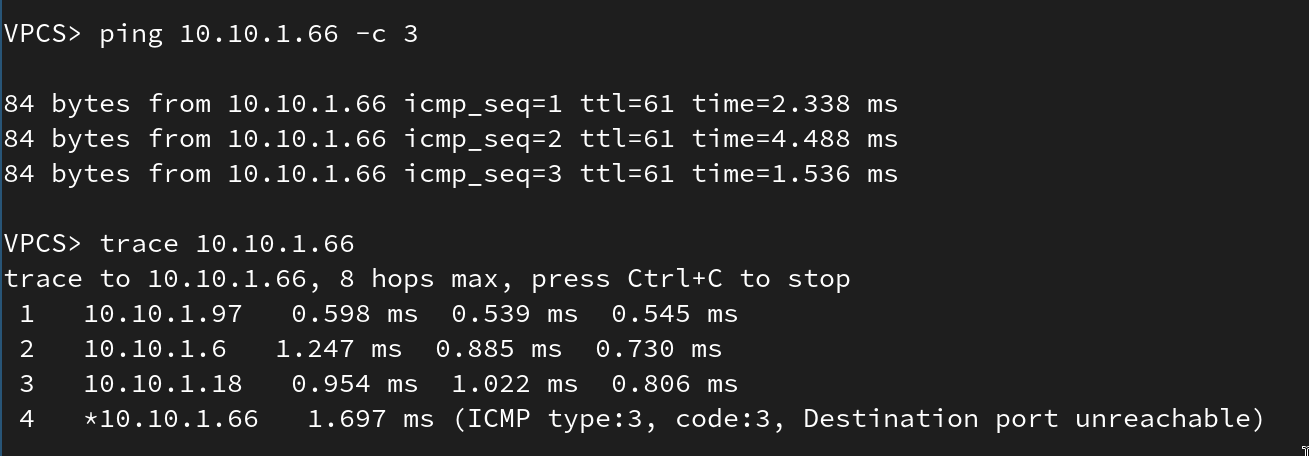
\includegraphics[width=0.8\textwidth]{../images/image102.png}
      \captionof{figure}{Проверка доступности PC1 с PC2.}
      \label{102}
    \end{center}

    \begin{center}
      \centering
      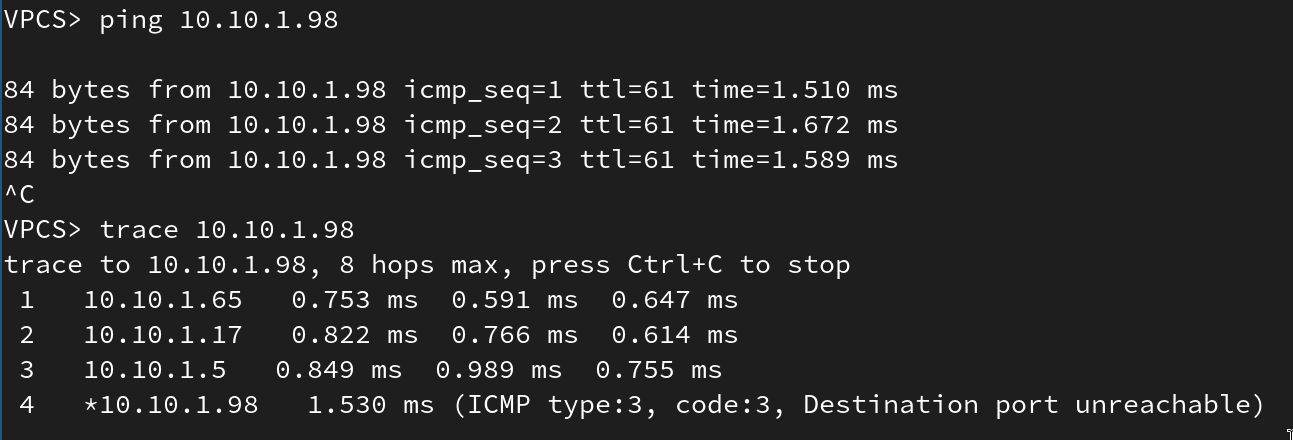
\includegraphics[width=0.8\textwidth]{../images/image103.png}
      \captionof{figure}{Проверка доступности PC2 с PC1.}
      \label{103}
    \end{center}

  \item Отключили интерфейс у маршрутизатора \texttt{msk-dastarikov-gw-03} и проверили, что маршрут восстановится по  маршрутизатору \texttt{msk-dastarikov-gw-04} (рис. \ref{104}-\ref{107}):

    \begin{center}
      \centering
      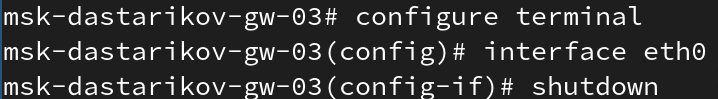
\includegraphics[width=0.8\textwidth]{../images/image104.png}
      \captionof{figure}{Отключение на маршрутизаторе \texttt{msk-dastarikov-gw-03} интерфейса \texttt{eth0}.}
      \label{104}
    \end{center}
    
    \begin{center}
      \centering
      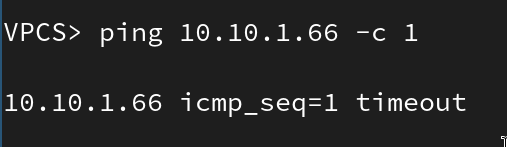
\includegraphics[width=0.8\textwidth]{../images/image105.png}
      \captionof{figure}{Отсутствие доступа после отключения интерфейса.}
      \label{105}
    \end{center}

    
    \begin{center}
      \centering
      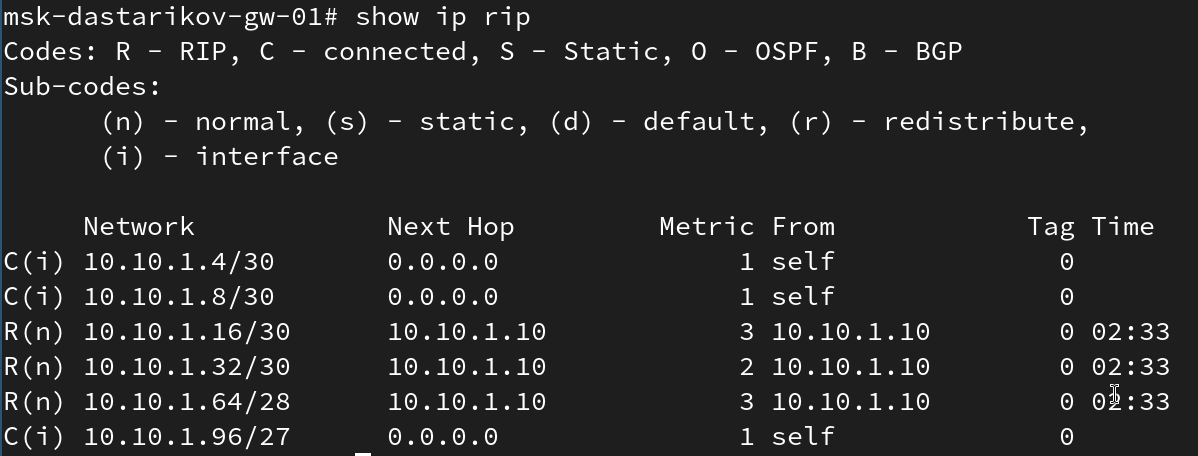
\includegraphics[width=0.8\textwidth]{../images/image106.png}
      \captionof{figure}{Просмотр таблицы маршрутизации RIP после отключения интерфейса.}
      \label{106}
    \end{center}

    \begin{center}
      \centering
      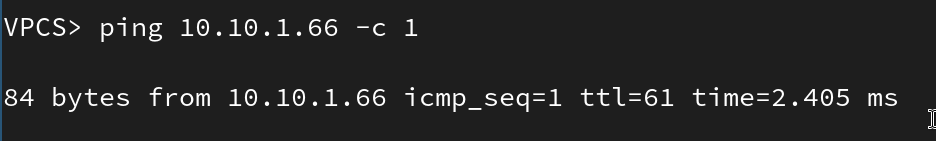
\includegraphics[width=0.8\textwidth]{../images/image107.png}
      \captionof{figure}{Восстановление доступа после отключения интерфейса.}
      \label{107}
    \end{center}

  \item Настроили динамическую маршрутизацию про протоколу RIPng (рис. \ref{109}-\ref{110}):

    \begin{center}
      \centering
      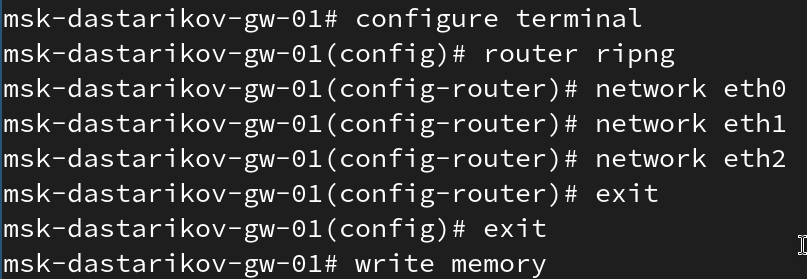
\includegraphics[width=0.8\textwidth]{../images/image109.png}
      \captionof{figure}{Настройка протокола RIPng на маршрутизатору \texttt{gw-01}.}
      \label{109}
    \end{center}

    \begin{center}
      \centering
      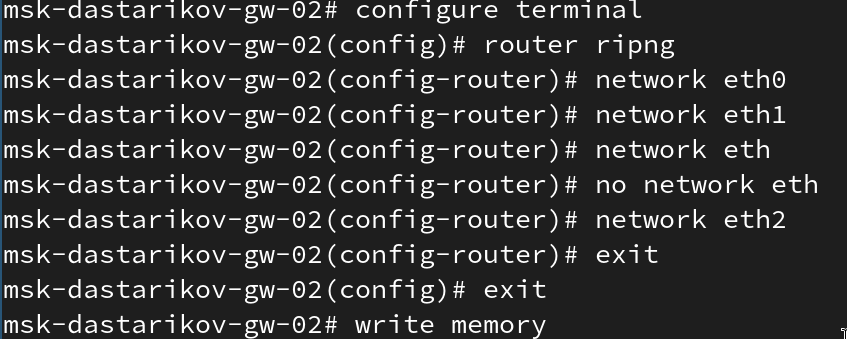
\includegraphics[width=0.8\textwidth]{../images/image108.png}
      \captionof{figure}{Настройка протокола RIPng на маршрутизатору \texttt{gw-02}.}
      \label{108}
    \end{center}

    \begin{center}
      \centering
      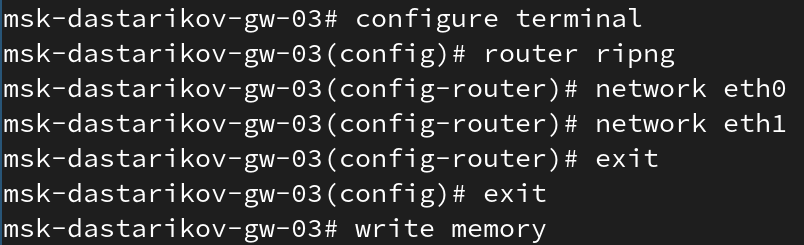
\includegraphics[width=0.8\textwidth]{../images/image110.png}
      \captionof{figure}{Настройка протокола RIPng на маршрутизатору \texttt{gw-03}.}
      \label{110}
    \end{center}

    \begin{center}
      \centering
      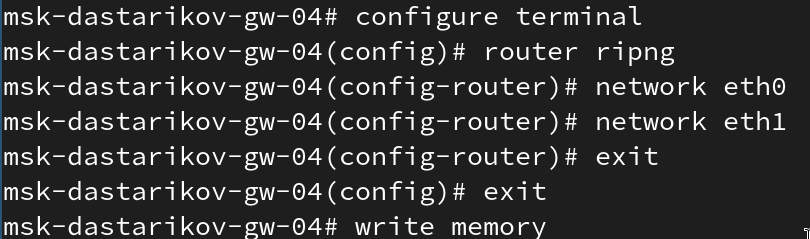
\includegraphics[width=0.8\textwidth]{../images/image111.png}
      \captionof{figure}{Настройка протокола RIPng на маршрутизатору \texttt{gw-04}.}
      \label{111}
    \end{center}

  \item Убедились, что маршрутизация по RIPng настроена (рис. \ref{114}):

    \begin{center}
      \centering
      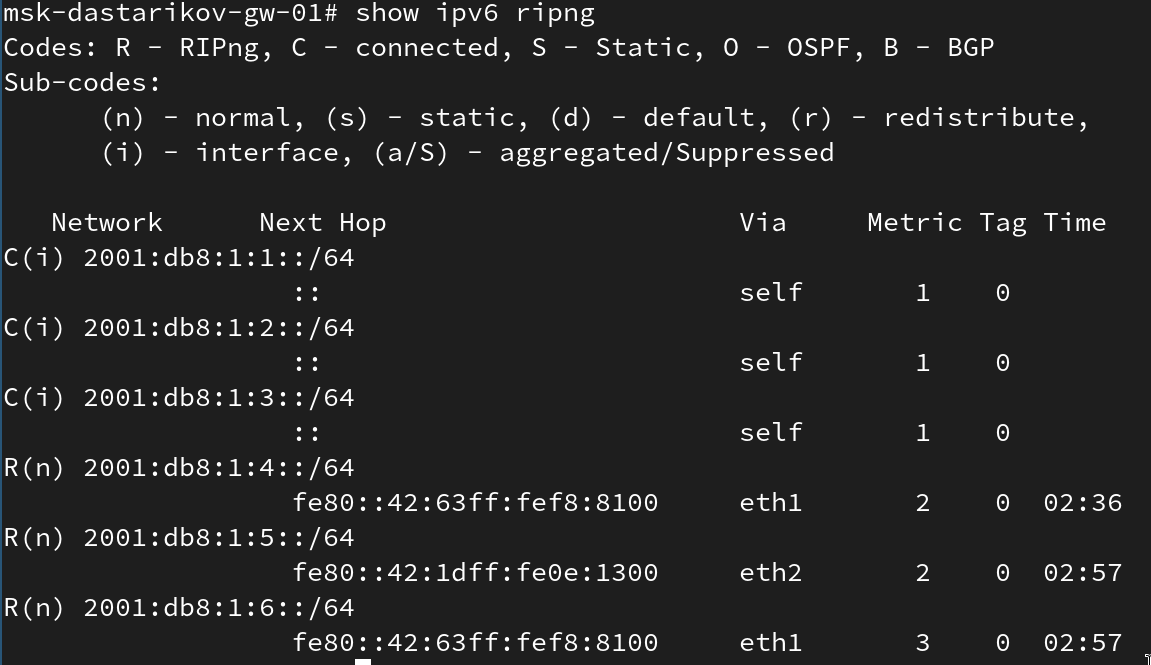
\includegraphics[width=0.8\textwidth]{../images/image114.png}
      \captionof{figure}{Просмотр настроек маршрутизации по RIPng.}
      \label{114}
    \end{center}


  \item Проверили доступность оконечных устройств (рис. \ref{112} и \ref{113}):

    \begin{center}
      \centering
      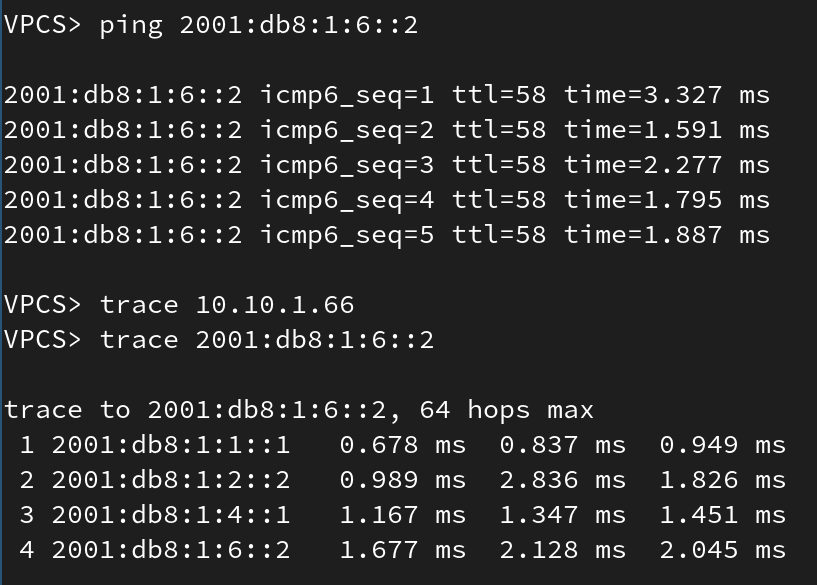
\includegraphics[width=0.8\textwidth]{../images/image112.png}
      \captionof{figure}{Проверка доступности PC1 с PC2.}
      \label{112}
    \end{center}

    \begin{center}
      \centering
      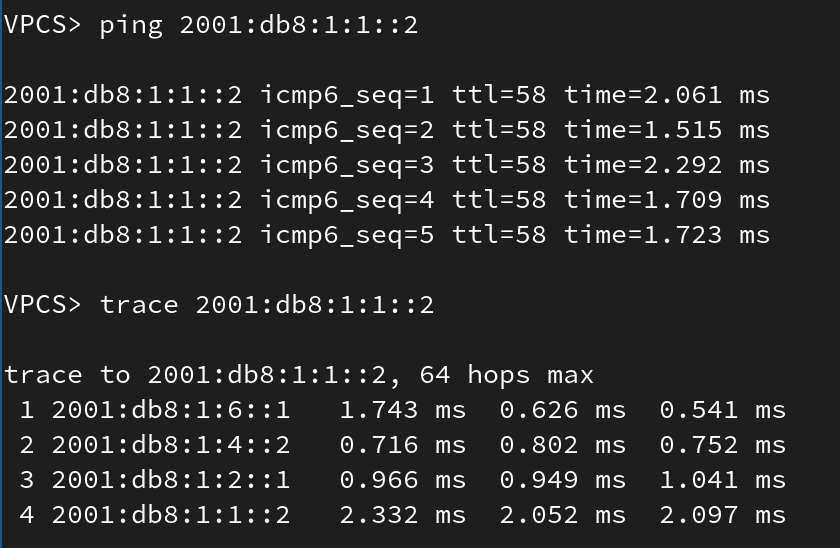
\includegraphics[width=0.8\textwidth]{../images/image113.png}
      \captionof{figure}{Проверка доступности PC2 с PC1.}
      \label{113}
    \end{center}

  \item Отключили интерфейс у маршрутизатора \texttt{msk-dastarikov-gw-03}, но доступ не восстановился. Устранить проблему не получилось (рис. \ref{115} и \ref{116}):

    \begin{center}
      \centering
      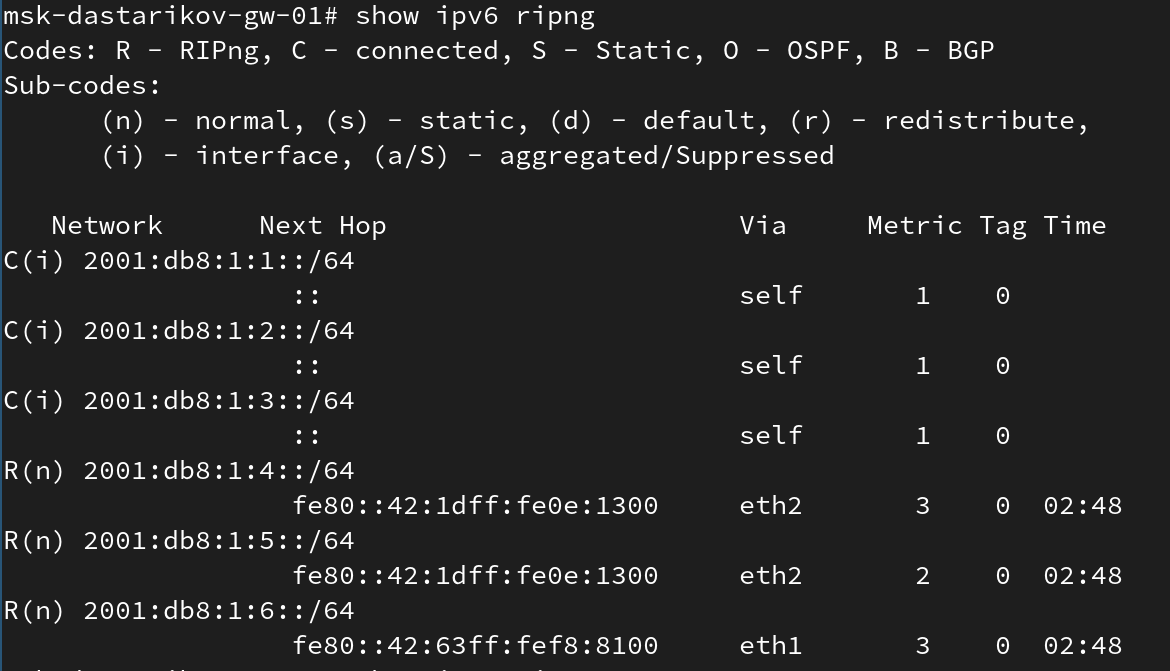
\includegraphics[width=0.8\textwidth]{../images/image115.png}
      \captionof{figure}{Просмотр настроек маршрутизации по RIPng после отключения интерфейса.}
      \label{115}
    \end{center}

    \begin{center}
      \centering
      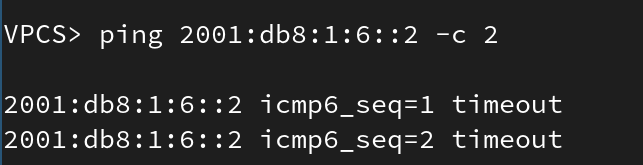
\includegraphics[width=0.8\textwidth]{../images/image116.png}
      \captionof{figure}{Отсутствие доступа после отключения интерфейса.}
      \label{116}
    \end{center}

  \item Настроили динамическую маршрутизацию по протокул OSPF (рис. \ref{117}-\ref{120}):

    \begin{center}
      \centering
      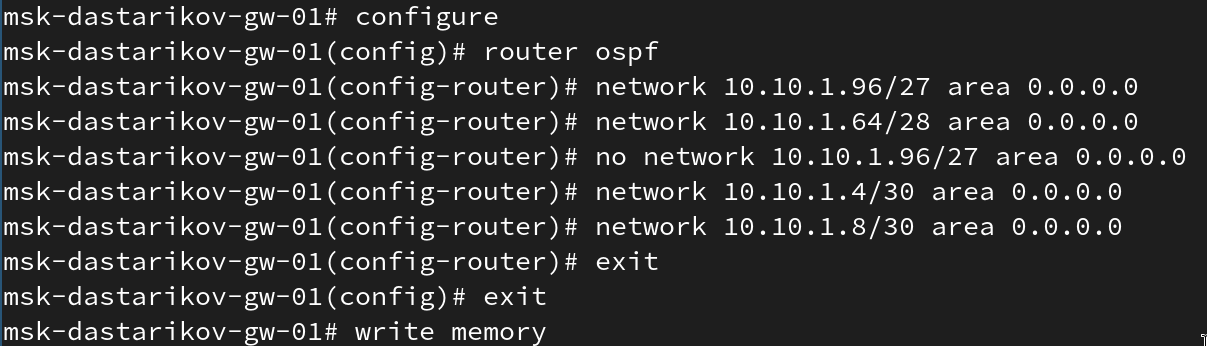
\includegraphics[width=0.8\textwidth]{../images/image117.png}
      \captionof{figure}{Настройка протокола OSPF на маршрутизатору \texttt{gw-01}.}
      \label{117}
    \end{center}

    \begin{center}
      \centering
      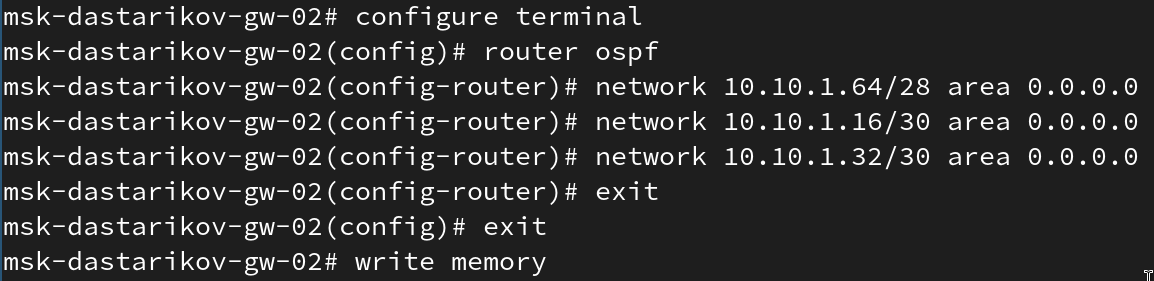
\includegraphics[width=0.8\textwidth]{../images/image118.png}
      \captionof{figure}{Настройка протокола OSPF на маршрутизатору \texttt{gw-02}.}
      \label{118}
    \end{center}

    \begin{center}
      \centering
      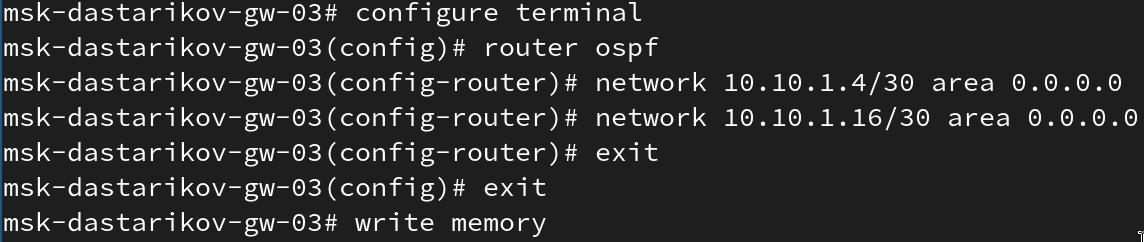
\includegraphics[width=0.8\textwidth]{../images/image119.png}
      \captionof{figure}{Настройка протокола OSPF на маршрутизатору \texttt{gw-03}.}
      \label{119}
    \end{center}

    \begin{center}
      \centering
      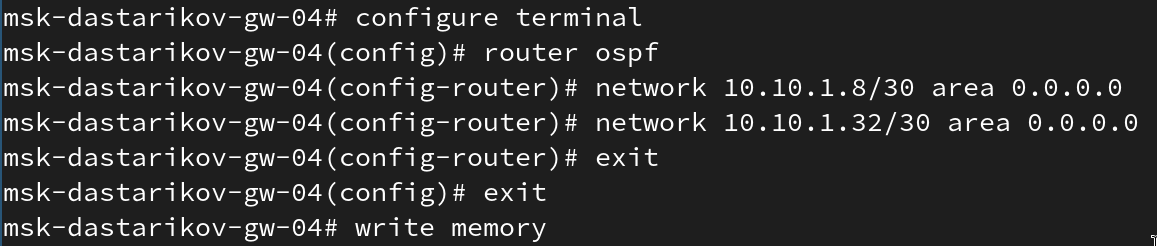
\includegraphics[width=0.8\textwidth]{../images/image120.png}
      \captionof{figure}{Настройка протокола OSPF на маршрутизатору \texttt{gw-04}.}
      \label{120}
    \end{center}

  \item Проверили доступность оконечных устройств (рис. \ref{121} и \ref{122}):

    \begin{center}
      \centering
      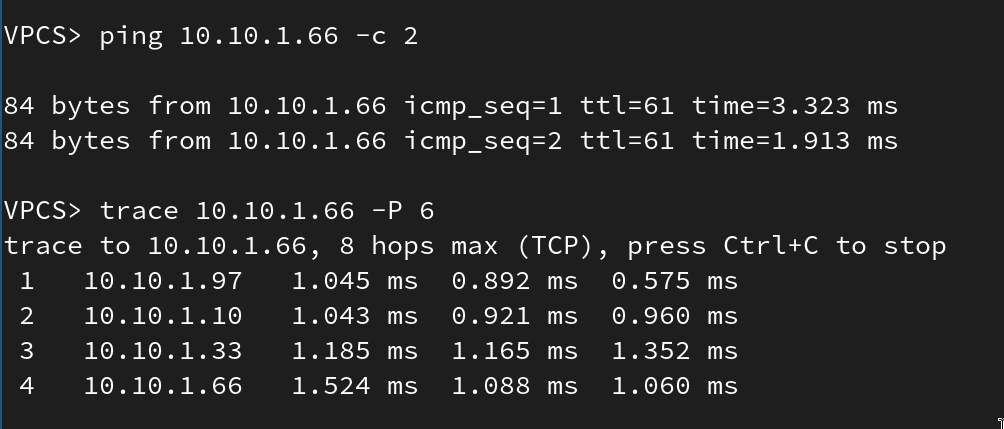
\includegraphics[width=0.8\textwidth]{../images/image121.png}
      \captionof{figure}{Проверка доступности PC1 с PC2.}
      \label{121}
    \end{center}

    \begin{center}
      \centering
      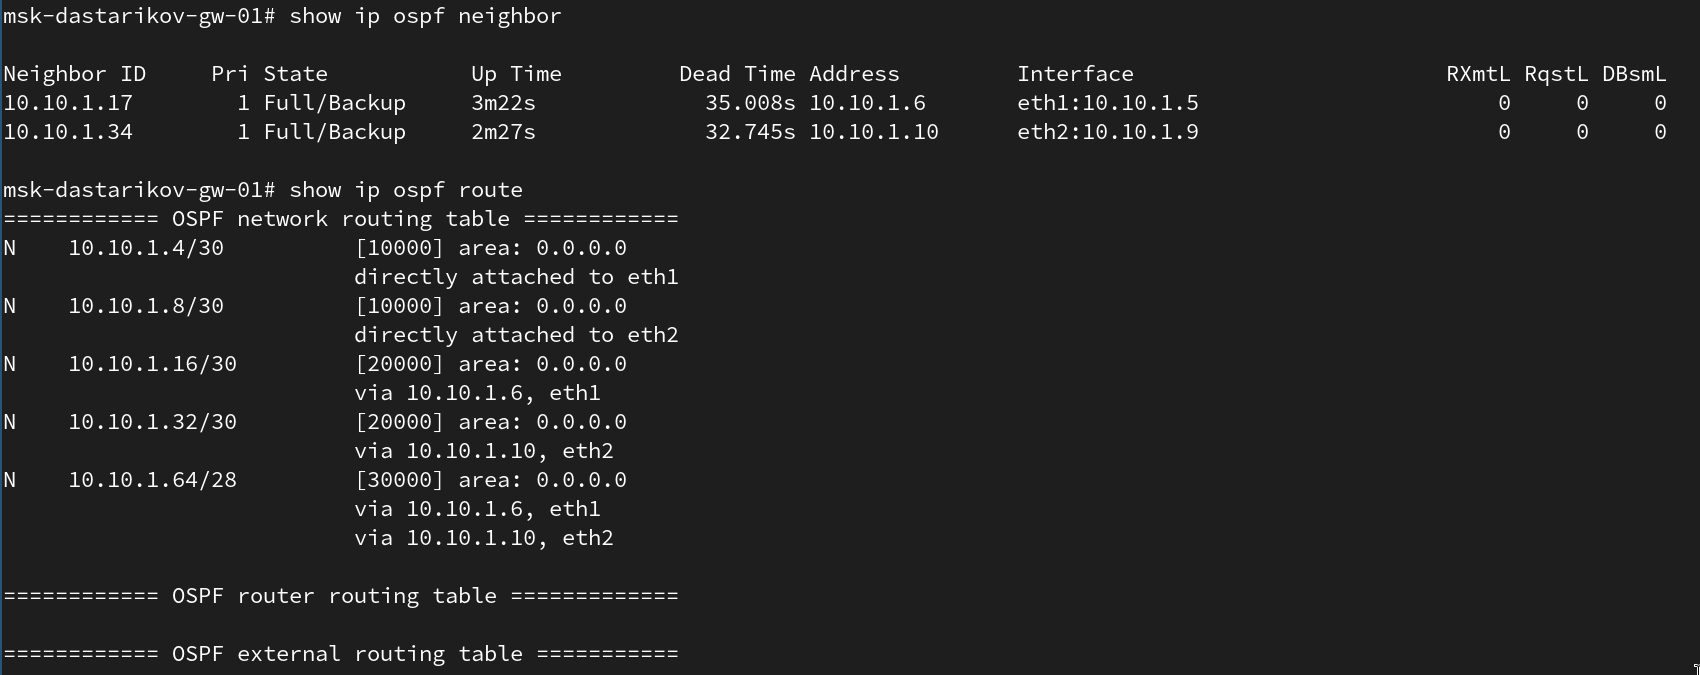
\includegraphics[width=0.8\textwidth]{../images/image122.png}
      \captionof{figure}{Просмотр настроек маршрутизации по OSPF.}
      \label{122}
    \end{center}

  \item Отключили интерфейс у маршрутизатора \texttt{msk-dastarikov-gw-04} и проверили, что маршрут восстановится по  маршрутизатору \texttt{msk-dastarikov-gw-03} (рис. \ref{123}-\ref{124}):

    \begin{center}
      \centering
      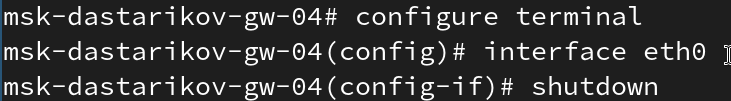
\includegraphics[width=0.8\textwidth]{../images/image123.png}
      \captionof{figure}{Отключение на маршрутизаторе \texttt{msk-dastarikov-gw-04} интерфейса \texttt{eth0}.}
      \label{123}
    \end{center}
    
    \begin{center}
      \centering
      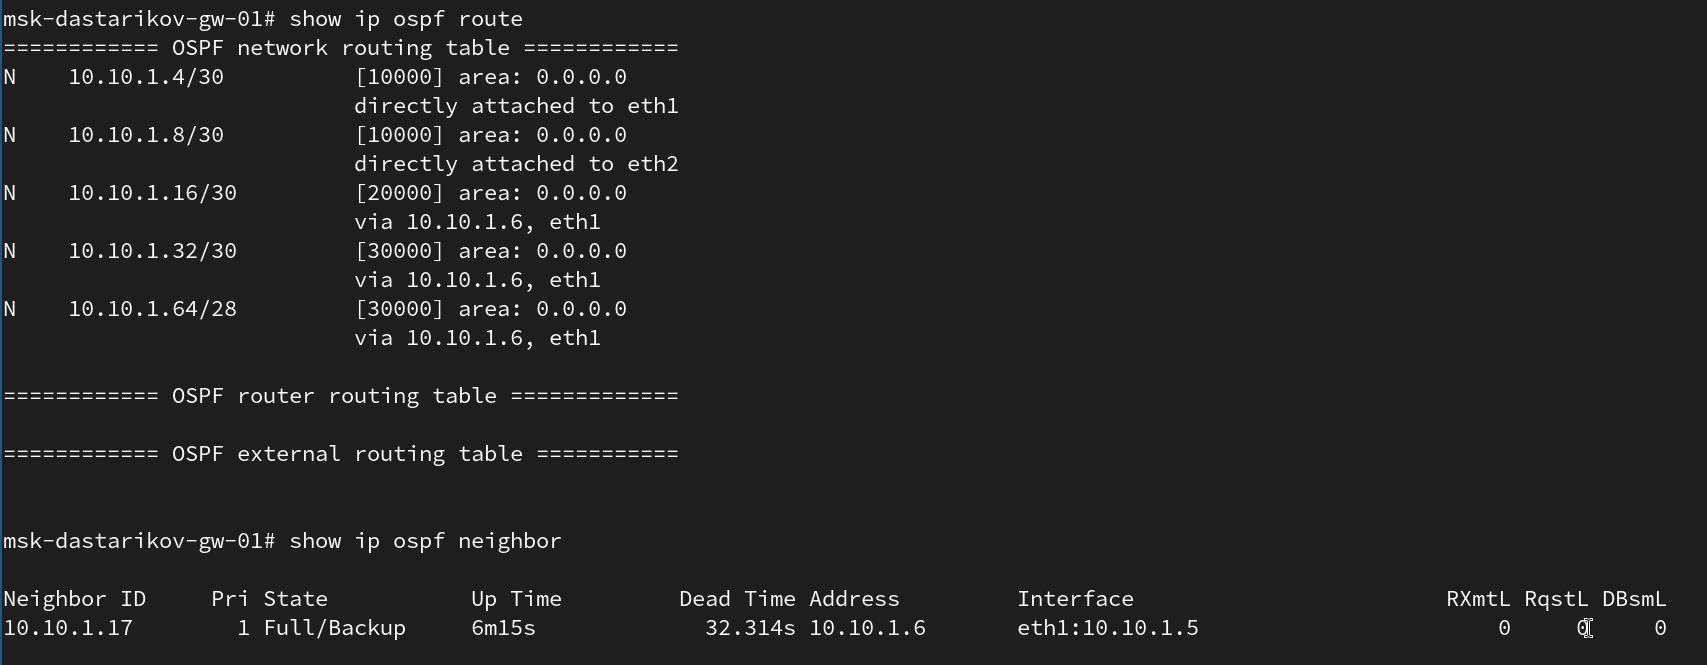
\includegraphics[width=0.8\textwidth]{../images/image125.png}
      \captionof{figure}{Просмотр таблицы маршрутизации OSPF после отключения интерфейса.}
      \label{125}
    \end{center}

    \begin{center}
      \centering
      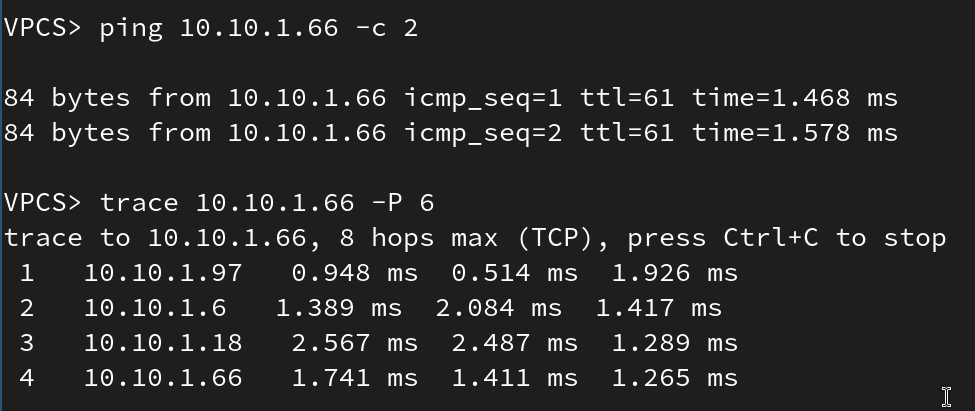
\includegraphics[width=0.8\textwidth]{../images/image124.png}
      \captionof{figure}{Восстановление доступа после отключения интерфейса.}
      \label{124}
    \end{center}

  \item Настроили динамическую маршрутизацию по протокул OSPFv3 (рис. \ref{126}-\ref{128}):

    \begin{center}
      \centering
      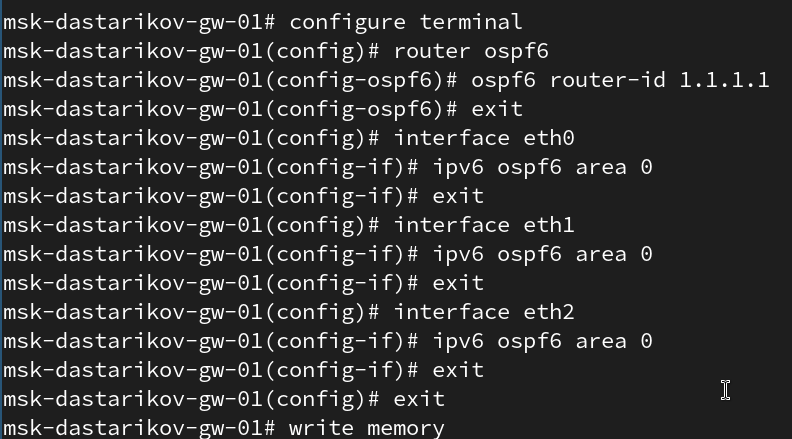
\includegraphics[width=0.8\textwidth]{../images/image126.png}
      \captionof{figure}{Настройка протокола OSPFv3 на маршрутизатору \texttt{gw-01}.}
      \label{126}
    \end{center}

    \begin{center}
      \centering
      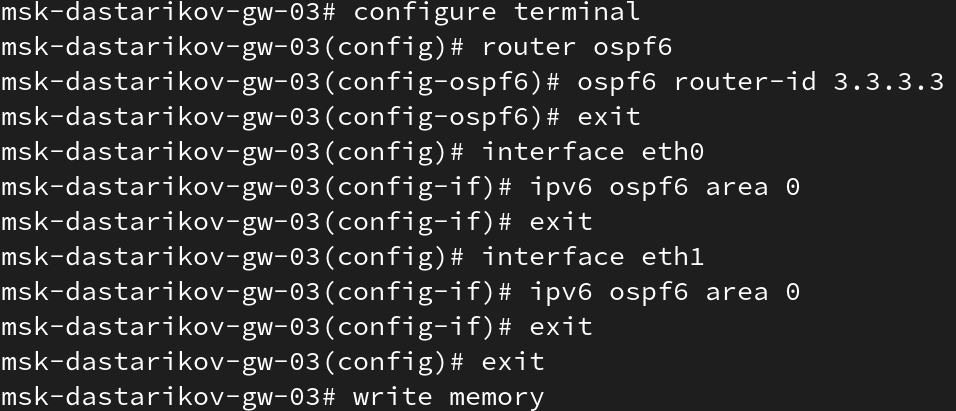
\includegraphics[width=0.8\textwidth]{../images/image127.png}
      \captionof{figure}{Настройка протокола OSPFv3 на маршрутизатору \texttt{gw-03}.}
      \label{127}
    \end{center}

    \begin{center}
      \centering
      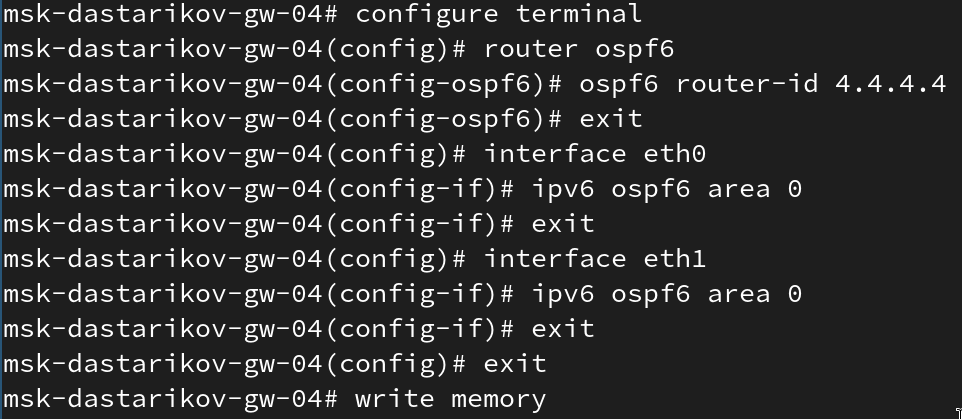
\includegraphics[width=0.8\textwidth]{../images/image128.png}
      \captionof{figure}{Настройка протокола OSPFv3 на маршрутизатору \texttt{gw-04}.}
      \label{128}
    \end{center}

  \item Проверили доступность оконечных устройств (рис. \ref{129}-\ref{130}):

    \begin{center}
      \centering
      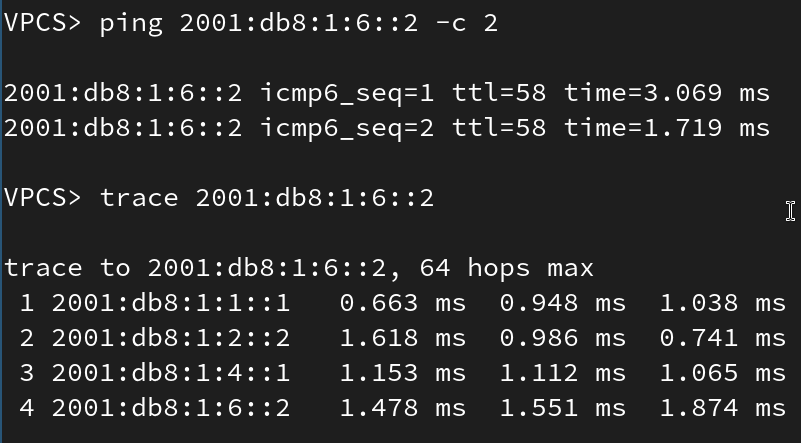
\includegraphics[width=0.8\textwidth]{../images/image129.png}
      \captionof{figure}{Проверка доступности PC1 с PC2.}
      \label{129}
    \end{center}

    \begin{center}
      \centering
      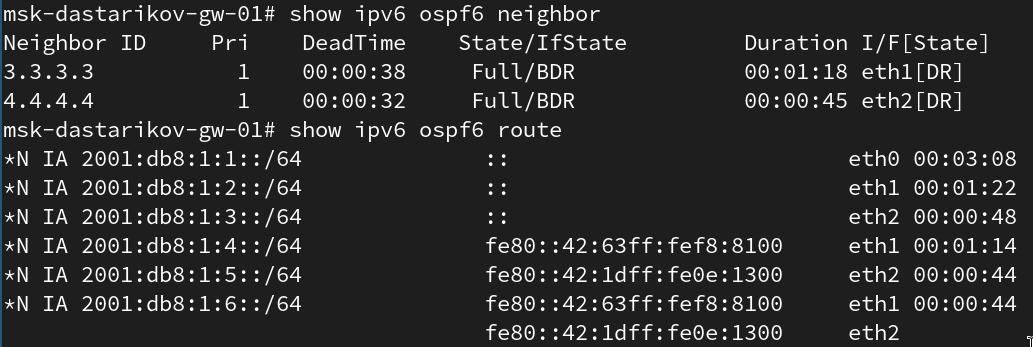
\includegraphics[width=0.8\textwidth]{../images/image130.png}
      \captionof{figure}{Просмотр настроек маршрутизации по OSPFv3.}
      \label{130}
    \end{center}


  \item Отключили интерфейс у маршрутизатора \texttt{msk-dastarikov-gw-04} и проверили, что маршрут восстановится по  маршрутизатору \texttt{msk-dastarikov-gw-03} (рис. \ref{132}-\ref{131}):
    
    \begin{center}
      \centering
      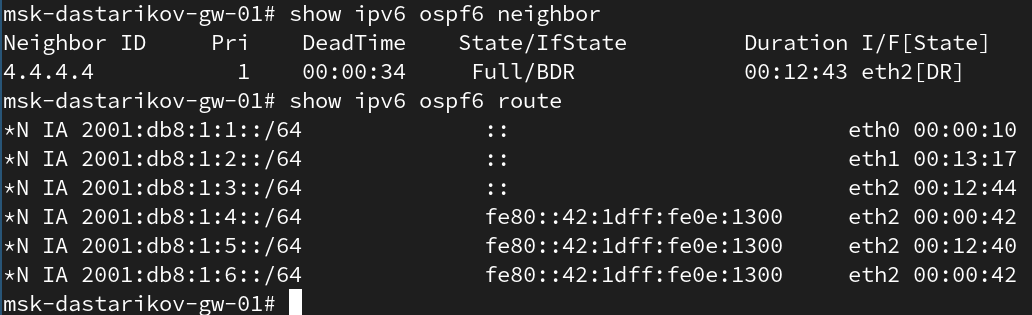
\includegraphics[width=0.8\textwidth]{../images/image132.png}
      \captionof{figure}{Просмотр таблицы маршрутизации OSPFv3 после отключения интерфейса.}
      \label{132}
    \end{center}

    \begin{center}
      \centering
      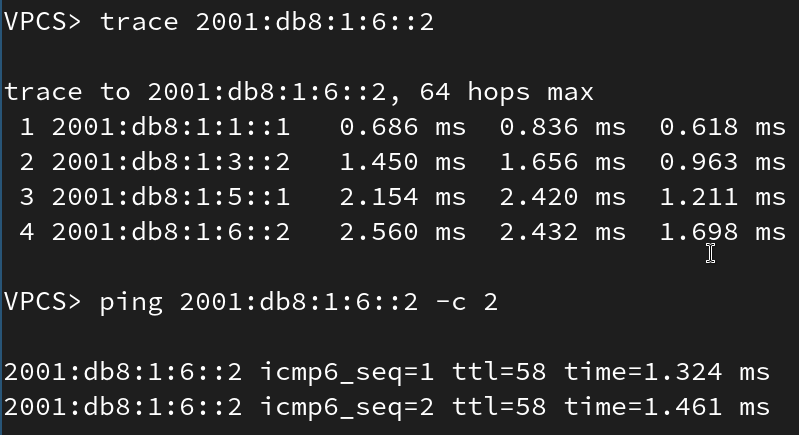
\includegraphics[width=0.8\textwidth]{../images/image131.png}
      \captionof{figure}{Восстановление доступа после отключения интерфейса.}
      \label{131}
    \end{center}

  \end{enumerate}
  \section{Выводы}
  В результате выполнения лабораторной работы изучили принципы маршрутизации в IPv4- и IPv6-сетях и принципы настройки сетевого оборудования. Самостоятельно настроили сеть с двойным стеком IPv4 и IPv6, динамической маршрутизацией для протоколов RIP и OSPF и проверили соединения и маршруты.
\end{document}
